% 第四部分：实验结果与分析
\section{实验结果与分析}

\begin{frame}{实验设计：数据集与任务范式}
    \begin{columns}[T]
        \begin{column}{0.55\textwidth}
            \begin{block}{\normalsize \textcolor{primaryblue}{BCI Competition IV 2a 数据集}}
                \begin{itemize}
                    \item \textbf{被试}：9 名健康被试
                    \item \textbf{任务}：4 类运动想象（左手、右手、脚、舌头）
                    \item \textbf{试次}：每类 72 次，共 288 试次/会话
                    \item \textbf{通道}：22 通道 EEG，10-20 系统
                    \item \textbf{采样率}：250 Hz
                \end{itemize}
            \end{block}
        \end{column}

        \begin{column}{0.45\textwidth}
            \begin{alertblock}{\normalsize 实验协议}
                \begin{itemize}
                    \item \textbf{训练集}：Session T（288 试次）
                    \item \textbf{测试集}：Session E（288 试次）
                    \item \textbf{重复实验}：5 次（随机种子 0-4）
                    \item \textbf{评估}：平均值 ± 标准差
                \end{itemize}
            \end{alertblock}
        \end{column}
    \end{columns}

    \vspace{0.5em}

    \begin{exampleblock}{\normalsize 评价指标}
        准确率 (Accuracy)、Cohen's Kappa、F1 分数、标准差 (Std Dev)、变异系数 (CV)
    \end{exampleblock}
\end{frame}

\begin{frame}{数据预处理与特征提取}
    \centering
    \begin{tikzpicture}[
        box/.style={rectangle, draw=primaryblue, fill=lightblue,
                   text width=4.5em, text centered, rounded corners=4pt,
                   minimum height=1.8em, font=\footnotesize, drop shadow},
        arrow/.style={->, >=Stealth, thick, primaryblue}
    ]
        \node[box] (raw) {原始 EEG};
        \node[box, right=0.5cm of raw] (bp) {带通滤波\\8-30 Hz};
        \node[box, right=0.5cm of bp] (notch) {陷波滤波\\50 Hz};
        \node[box, right=0.5cm of notch] (car) {平均参考};
        \node[box, right=0.5cm of car] (window) {时间窗截取};

        \draw[arrow] (raw) -- (bp);
        \draw[arrow] (bp) -- (notch);
        \draw[arrow] (notch) -- (car);
        \draw[arrow] (car) -- (window);
    \end{tikzpicture}

    \vspace{0.8em}

    \begin{columns}[T]
        \begin{column}{0.48\textwidth}
            \begin{block}{\normalsize \textcolor{primaryblue}{CSP 特征提取}}
                \begin{itemize}
                    \item 4 个 CSP 分量
                    \item 对数方差特征
                    \item Z-score 标准化
                \end{itemize}
            \end{block}
        \end{column}

        \begin{column}{0.48\textwidth}
            \begin{block}{\normalsize \textcolor{accentgreen}{SVM 分类器}}
                \begin{itemize}
                    \item 线性核函数
                    \item $C = 1.0$
                    \item 5 折交叉验证
                \end{itemize}
            \end{block}
        \end{column}
    \end{columns}
\end{frame}

\begin{frame}{对比方法}
    \begin{columns}[T]
        \begin{column}{0.32\textwidth}
            \begin{block}{\centering \normalsize 固定时间窗}
                \begin{itemize}
                    \item \textbf{FL-2s}：2.0s 固定长度
                    \item \textbf{FL-1.5s}：1.5s 固定长度
                    \item \textbf{FL-1s}：1.0s 固定长度
                \end{itemize}
            \end{block}
        \end{column}

        \begin{column}{0.32\textwidth}
            \begin{block}{\centering \normalsize 搜索优化}
                \begin{itemize}
                    \item \textbf{Grid-Search}：网格搜索（步长 0.2s）
                    \item \textbf{Random-Search}：随机采样 50 个
                \end{itemize}
            \end{block}
        \end{column}

        \begin{column}{0.32\textwidth}
            \begin{block}{\centering \normalsize 强化学习}
                \begin{itemize}
                    \item \textbf{Standard Q-Learning}
                    \item \textbf{Double Q-Learning}
                    \item \textbf{Dueling Q-Learning}
                    \item \textbf{Dueling Double Q}
                    \item \textbf{DQN}
                \end{itemize}
            \end{block}
        \end{column}
    \end{columns}

    \vspace{0.5em}

    \begin{alertblock}{\normalsize 实验层次}
        \begin{enumerate}
            \item \textbf{基线对比}：自适应 vs 固定时间窗
            \item \textbf{Q-Learning vs 基线}：强化学习 vs 搜索优化
            \item \textbf{Table Q vs DQN}：表格型 vs 深度强化学习
            \item \textbf{消融实验}：Q-Learning 变体对比
        \end{enumerate}
    \end{alertblock}
\end{frame}

% ==================== 基线方法性能对比 ====================
\begin{frame}{基线方法性能对比}
    \centering
    \vspace{-0.5em}
    \begin{table}
        \centering
        \Large
        \begin{tabular}{lcccc}
            \toprule
            \textbf{Method} & \textbf{Acc (\%)} & \textbf{Kappa} & \textbf{F1} & \textbf{Std (\%)} \\
            \midrule
            Fixed-2s & 45.08 & 0.2662 & 0.4255 & 8.95 \\
            \rowcolor{lightblue}
            Fixed-1.5s & 45.05 & 0.2659 & 0.4253 & 10.19 \\
            Fixed-1s & 45.47 & 0.2721 & 0.4344 & 10.87 \\
            \rowcolor{lightblue}
            Random-Search & 61.95 & 0.4920 & 0.6106 & 8.38 \\
            Grid-Search & \textbf{63.35} & \textbf{0.5107} & \textbf{0.6252} & 8.78 \\
            \bottomrule
        \end{tabular}
    \end{table}

\end{frame}

\begin{frame}{基线方法性能对比（可视化）}
    \centering
    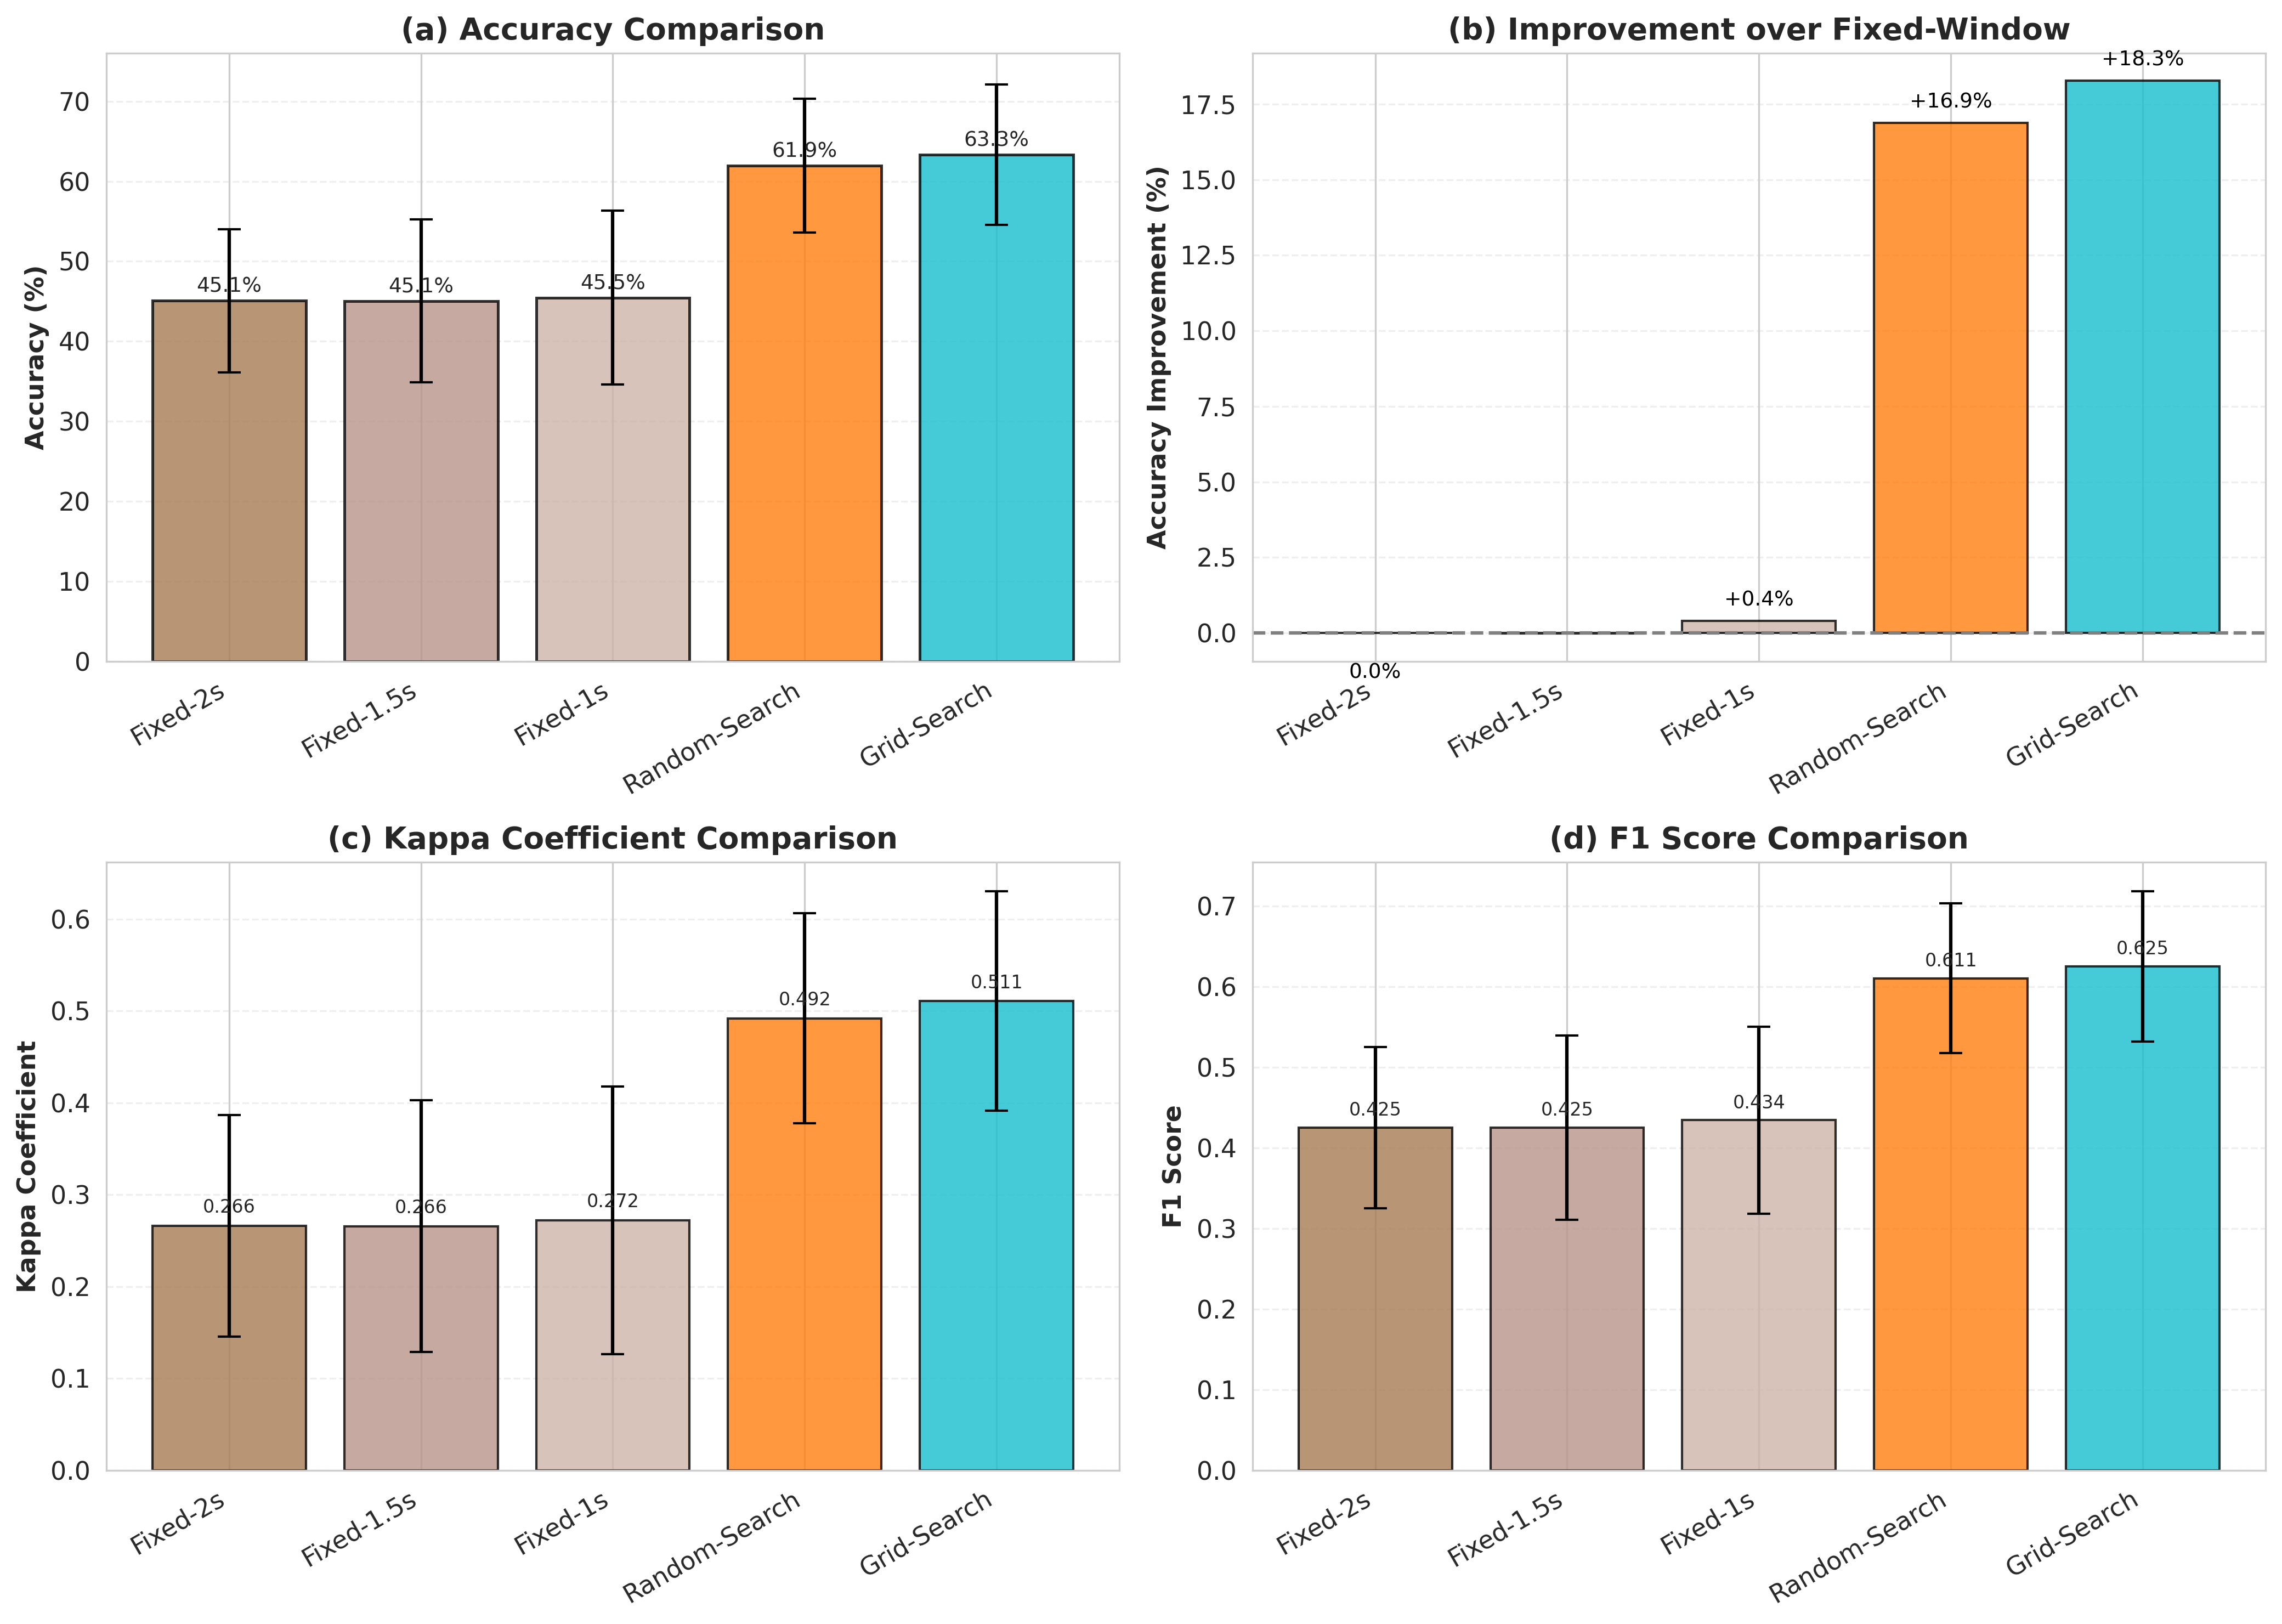
\includegraphics[height=0.8\textheight]{figures/baseline/01_performance_comparison.png}
\end{frame}

\begin{frame}{基线方法稳定性分析}
    \begin{columns}[T]
        \begin{column}{0.5\textwidth}
            \centering
            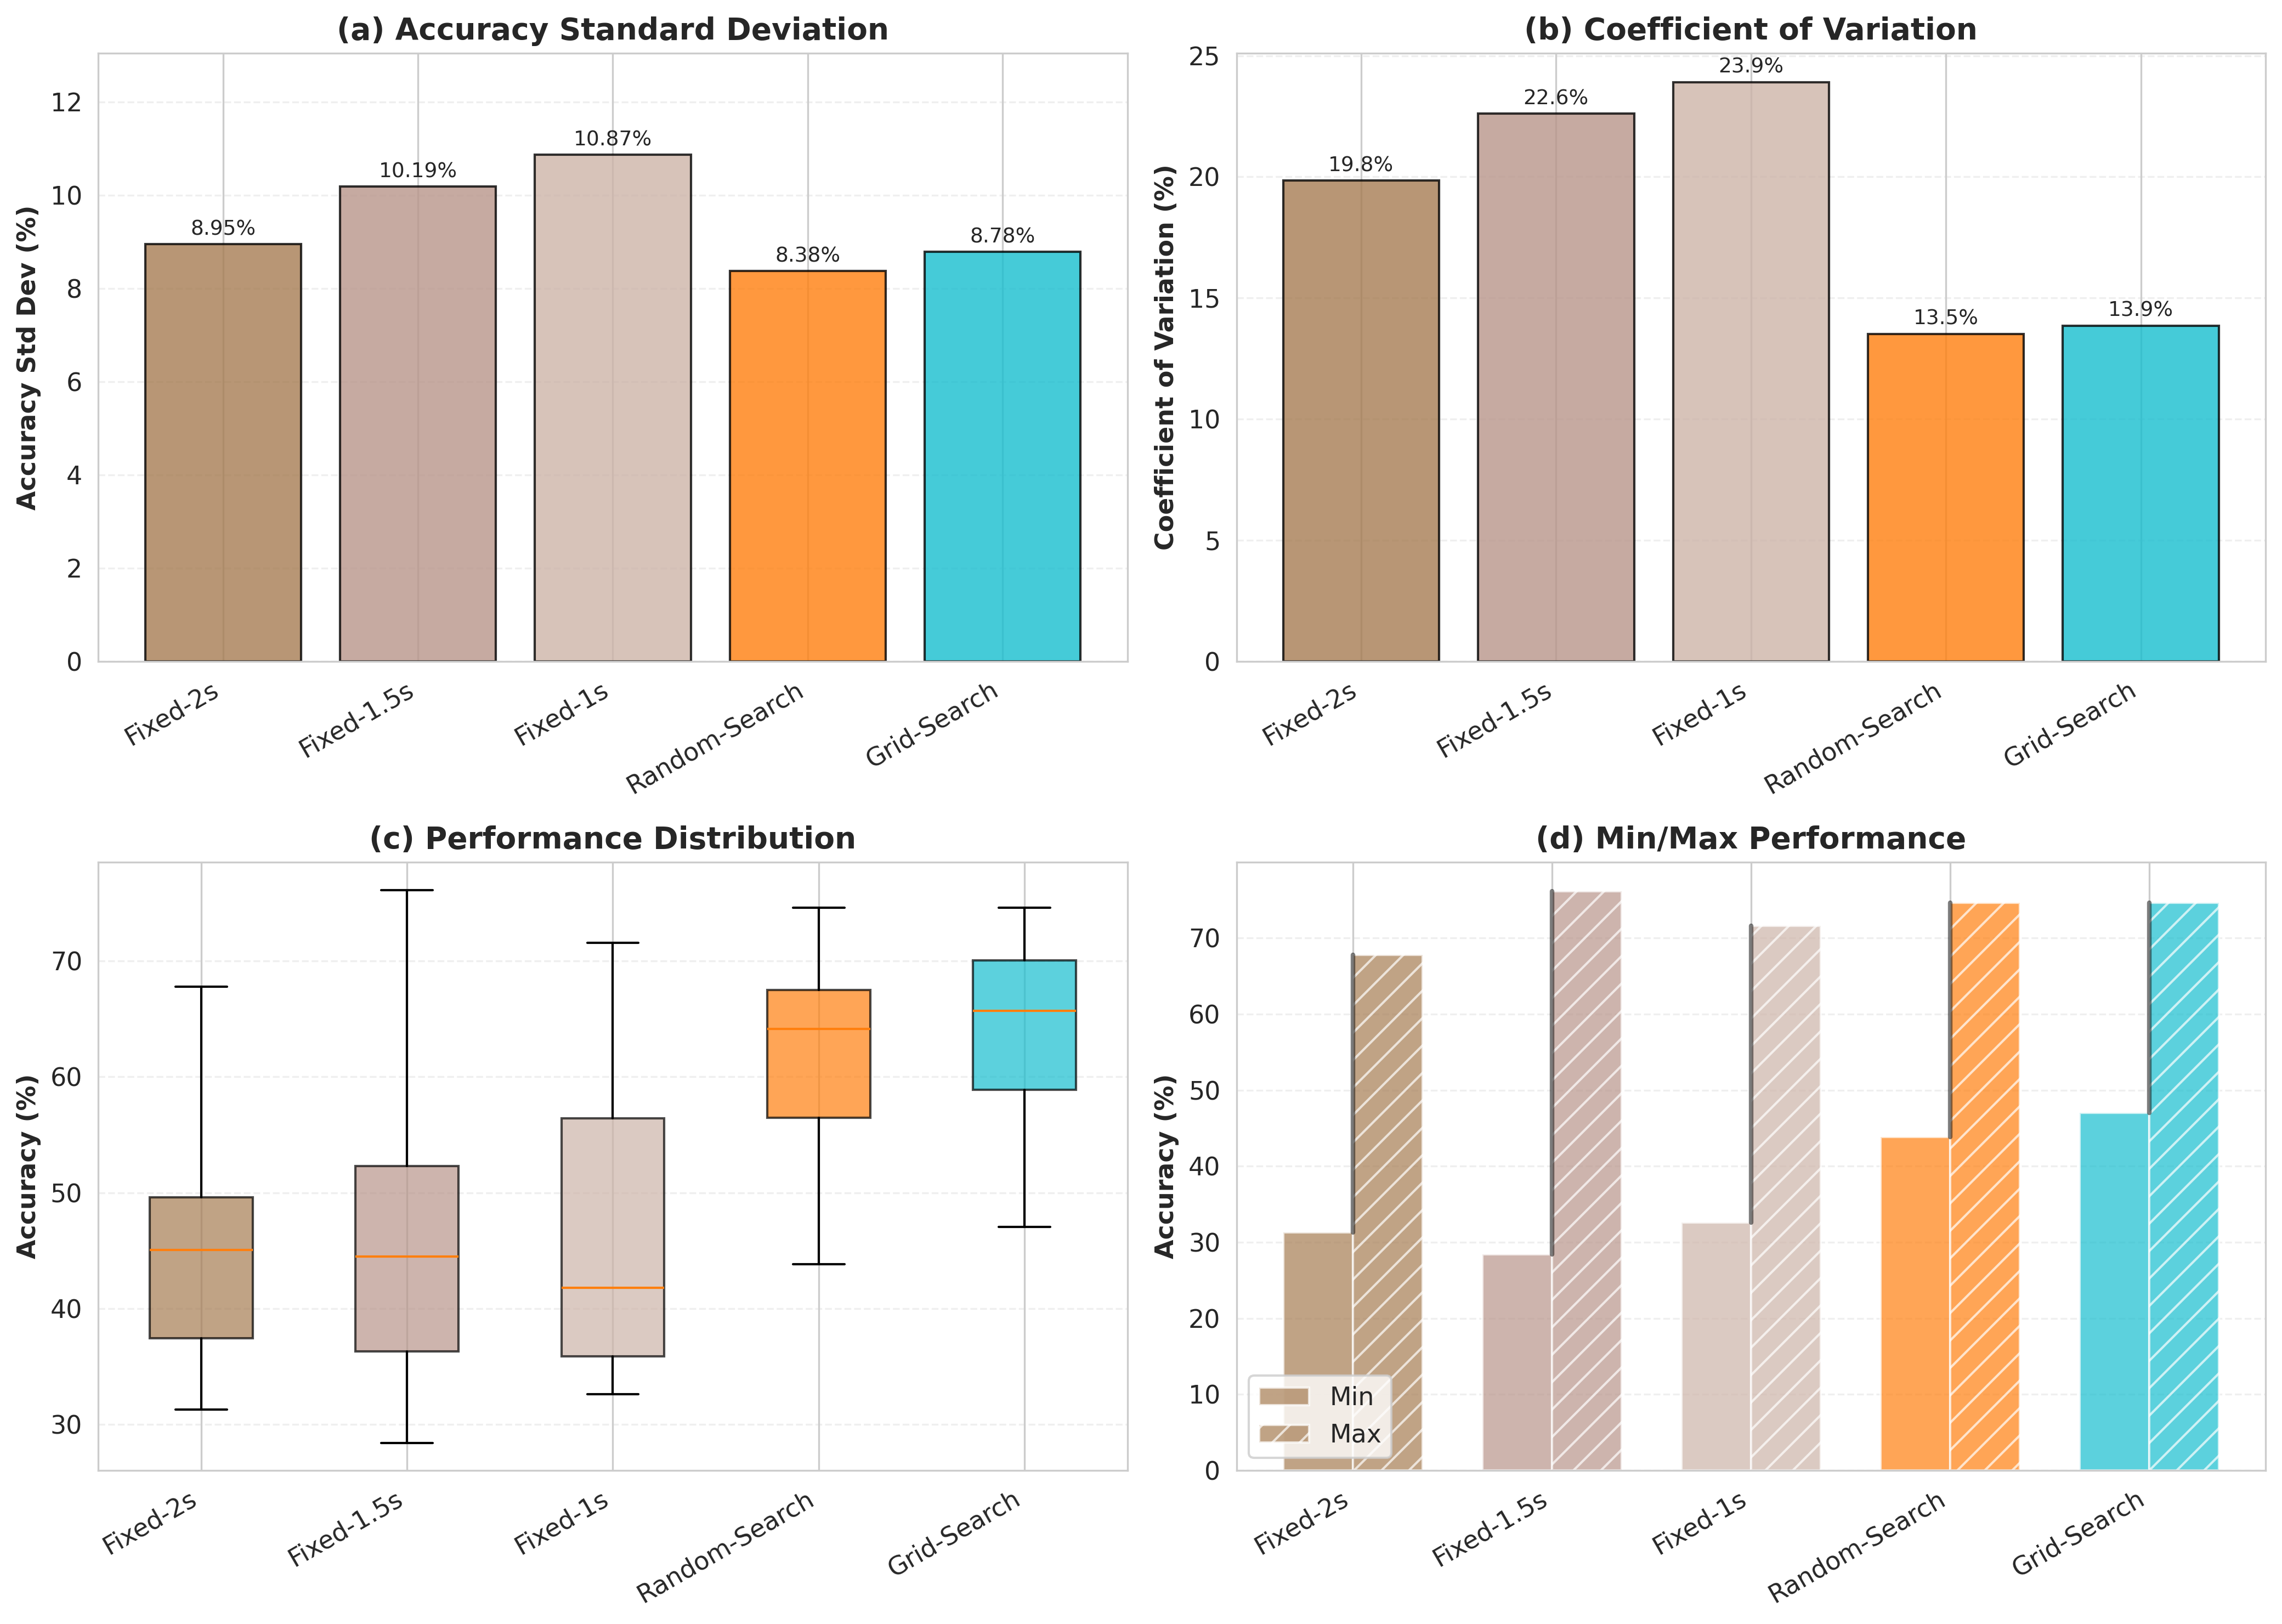
\includegraphics[height=0.7\textheight]{figures/baseline/01_stability_analysis.png}
            \vspace{-0.5em}
            \parbox{0.9\textwidth}{\footnotesize 图：基线方法稳定性箱线图}
        \end{column}

        \begin{column}{0.5\textwidth}
            \centering
            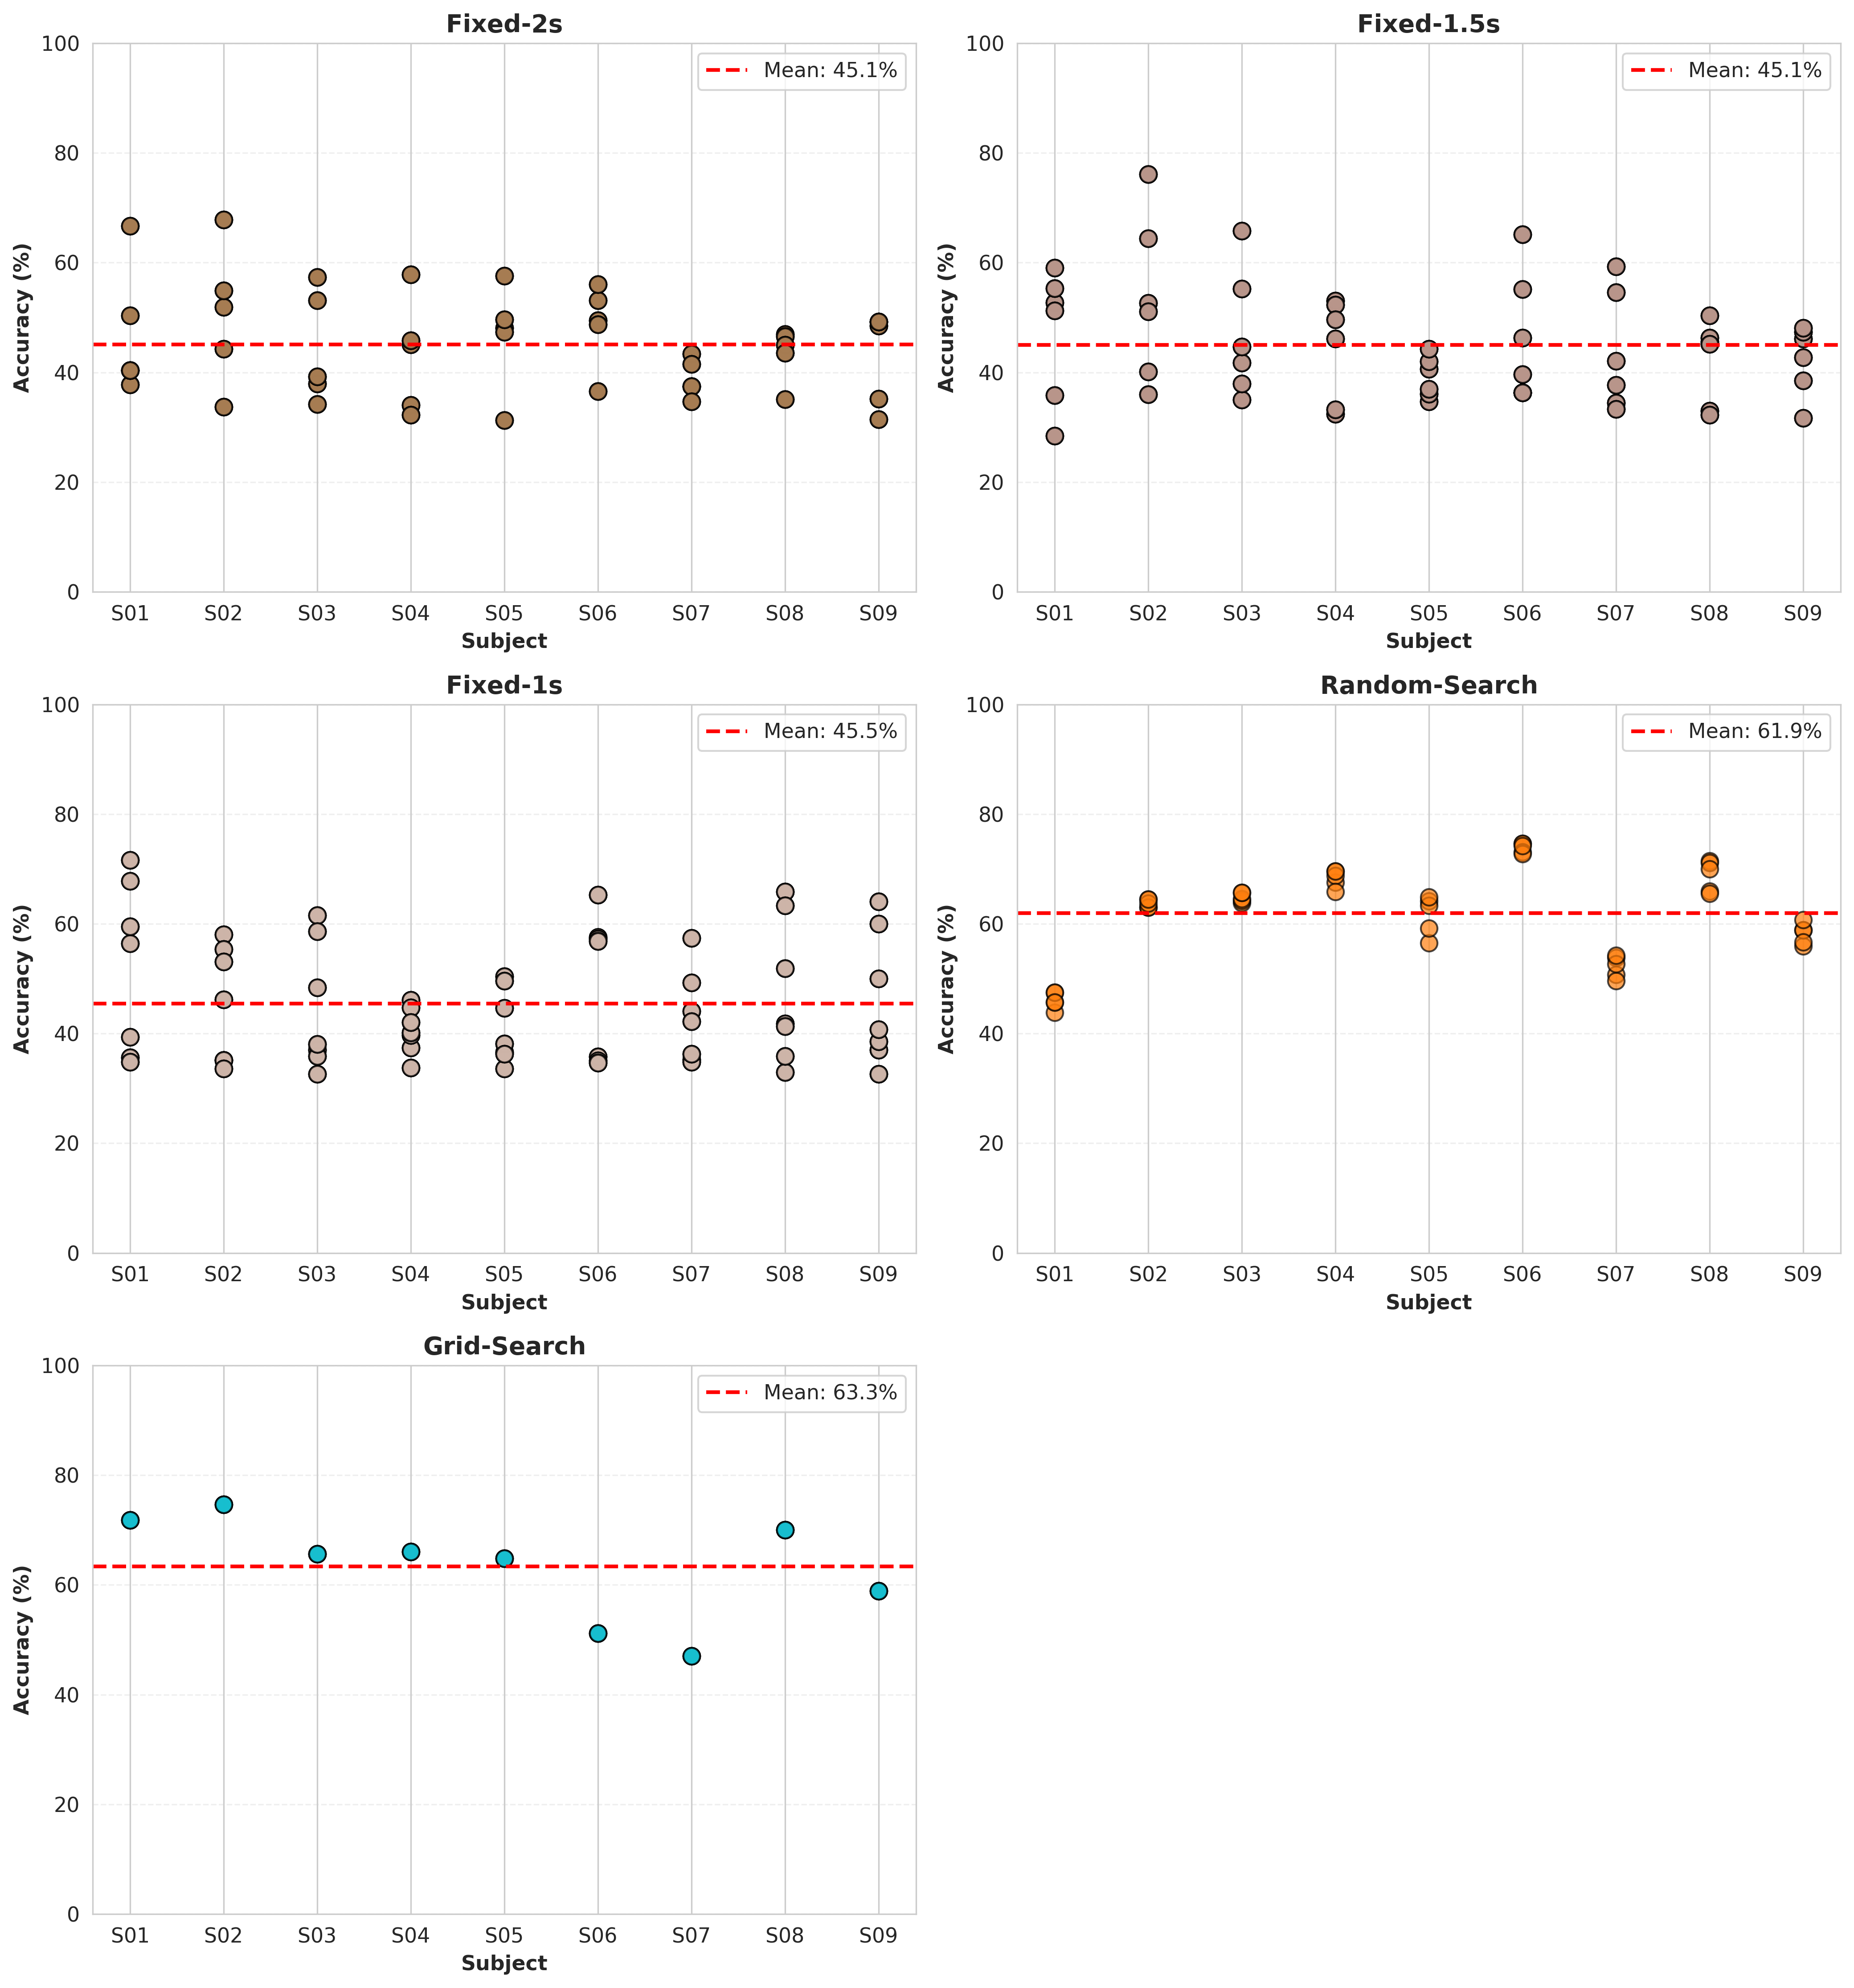
\includegraphics[height=0.7\textheight]{figures/baseline/01_subject_distribution.png}
            \vspace{-0.5em}
            \parbox{0.9\textwidth}{\footnotesize 图：被试级别性能热力图}
        \end{column}
    \end{columns}


\end{frame}

% ==================== Q-Learning 与基线方法对比 ====================
\begin{frame}{Q-Learning 方法与基线方法整体对比}
    \centering
    \vspace{-0.5em}
    \begin{table}
        \centering
        \begin{tabular}{lccccc}
            \toprule
            \textbf{Method} & \textbf{Acc (\%)} & \textbf{Kappa} & \textbf{F1} & \textbf{Std (\%)} & \textbf{$t_{start}$} \\
            \midrule
            Grid-Search & \textbf{63.35} & \textbf{0.5107} & \textbf{0.6252} & 8.78 & 2.27 \\
            \rowcolor{lightblue}
            \textbf{\color{primaryblue}Standard Q-Learning} & \textbf{62.68} & \textbf{0.5019} & \textbf{0.6201} & \textbf{8.20} & 2.29 \\
            Dueling Q-Learning & 62.74 & 0.5029 & 0.6204 & 8.26 & 2.27 \\
            \rowcolor{lightblue}
            DQN & 62.70 & 0.5022 & 0.6200 & 9.21 & 2.23 \\
            Double Q-Learning & 61.86 & 0.4909 & 0.6103 & 8.42 & 2.17 \\
            \rowcolor{lightblue}
            Dueling Double Q & 61.73 & 0.4894 & 0.6094 & 9.11 & 2.17 \\
            Random-Search & 61.95 & 0.4920 & 0.6106 & 8.38 & 2.20 \\
            \bottomrule
        \end{tabular}
    \end{table}


    \begin{alertblock}{\normalsize 核心发现}
        \begin{itemize}
            \item \textbf{Standard Q-Learning 稳定性最优}：Std Dev = 8.20\%（所有方法最低）
            \item \textbf{与 Grid-Search 性能接近}：Δ = -0.67\%，但计算成本更低
            \item \textbf{复杂变体未带来收益}：Double/Dueling 性能反而下降
        \end{itemize}
    \end{alertblock}
\end{frame}

\begin{frame}{Q-Learning 与基线方法对比（可视化）}
    \centering
    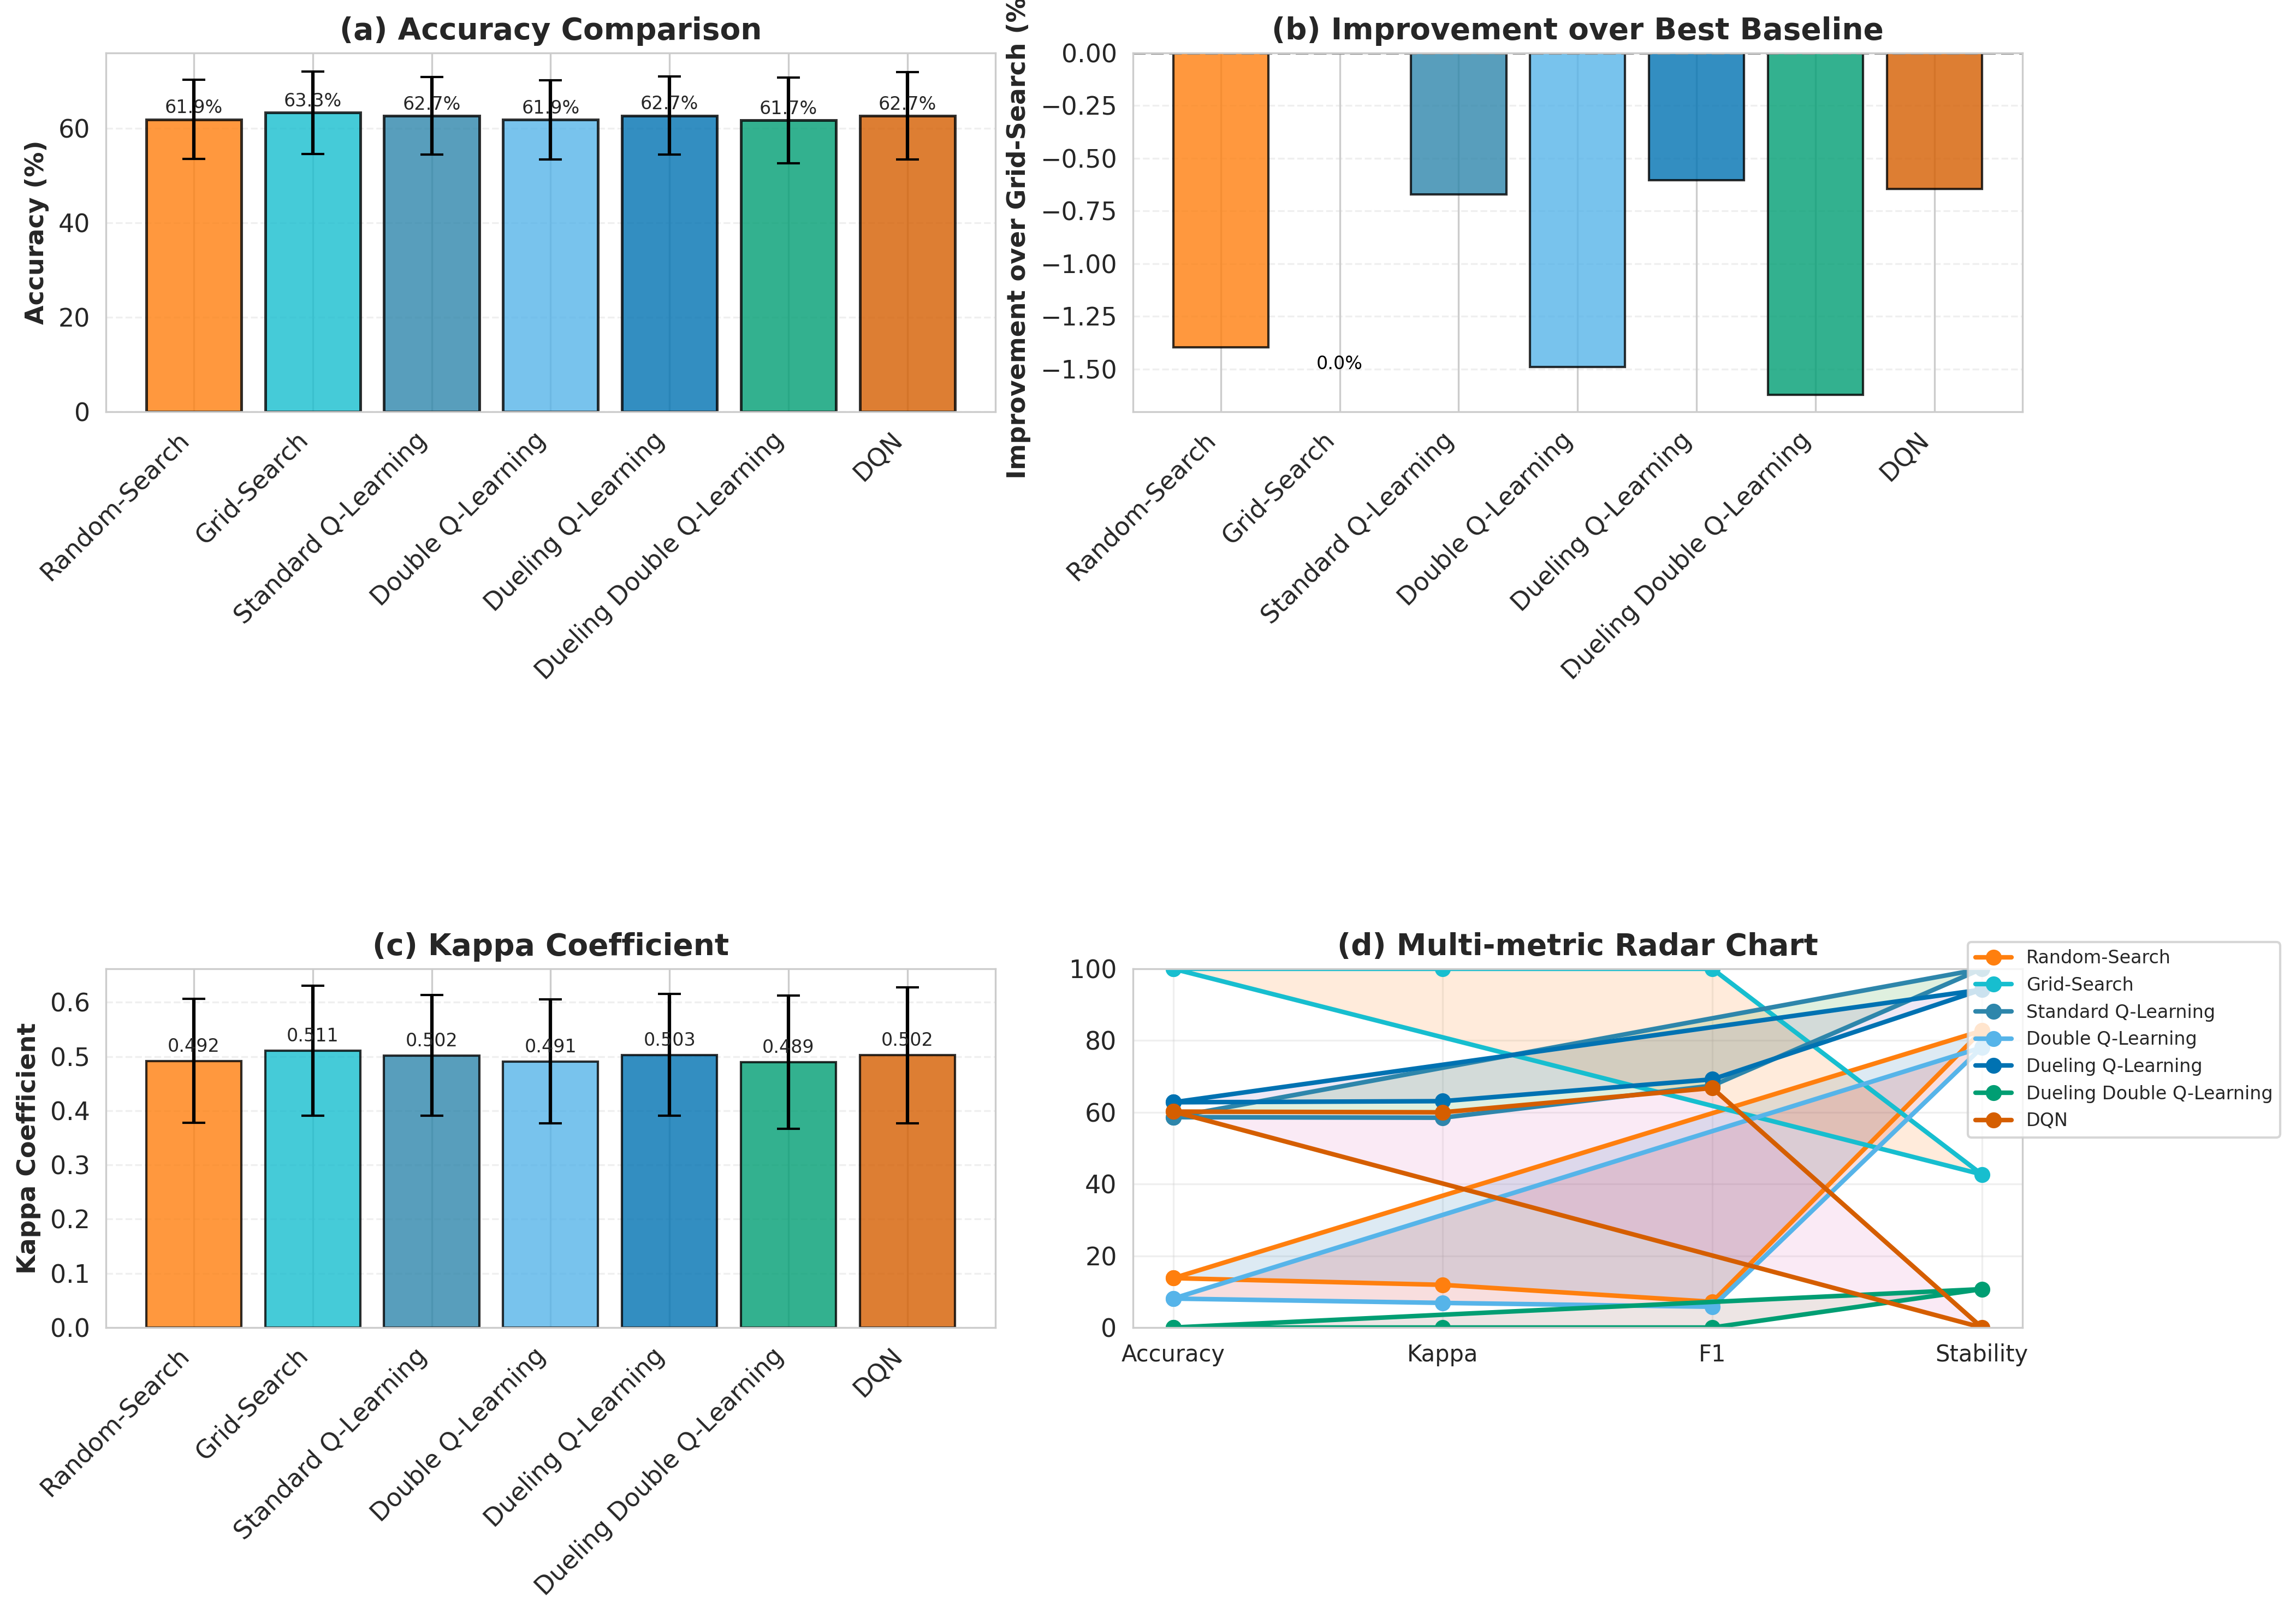
\includegraphics[height=0.7\textheight]{figures/q_vs_baseline/02_performance_comparison.png}
    \vspace{0.3em}
    \parbox{0.8\textwidth}{\footnotesize 图：Q-Learning 与基线方法性能对比}
\end{frame}

\begin{frame}{效应量分析与性能排名}
    \begin{columns}[T]
        \begin{column}{0.55\textwidth}
            \centering
            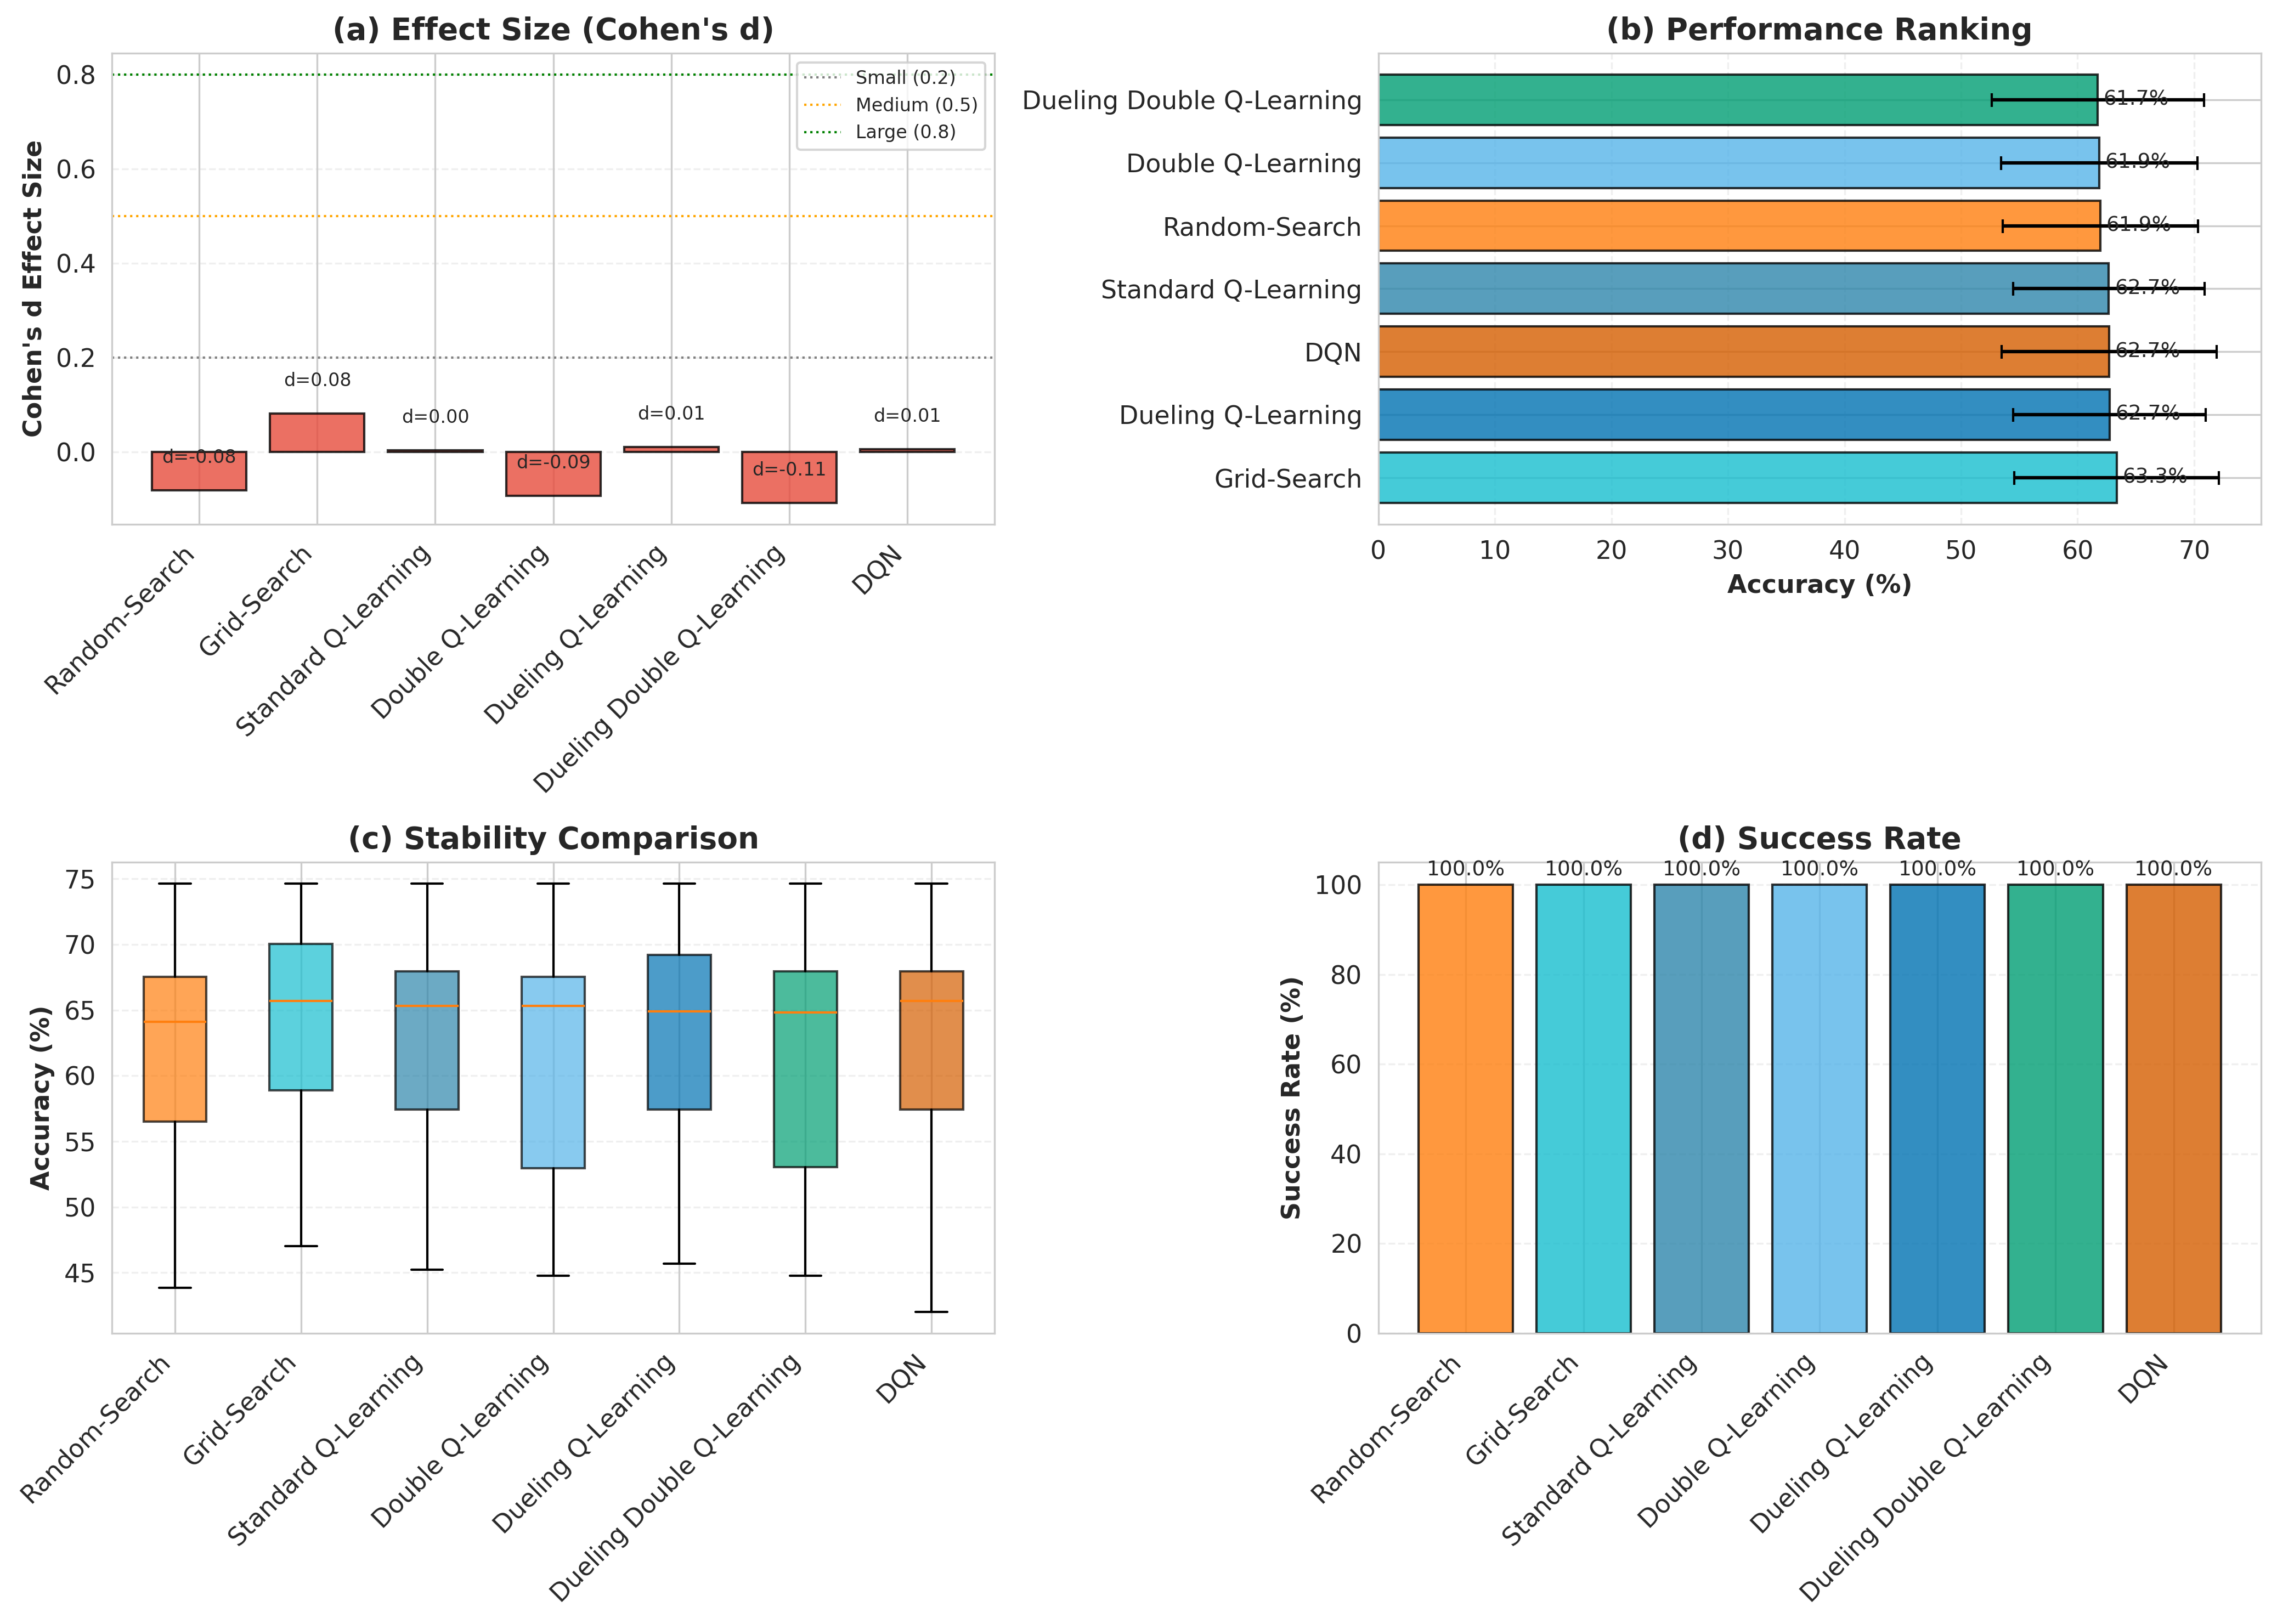
\includegraphics[height=0.6\textheight]{figures/q_vs_baseline/02_statistical_analysis.png}
            \vspace{-0.5em}
            \parbox{0.9\textwidth}{\footnotesize 图：Cohen's d 效应量与性能排名}
        \end{column}

        \begin{column}{0.45\textwidth}
            \begin{block}{\normalsize 效应量分析}
                以 Standard Q-Learning 为基准：
                \begin{itemize}
                    \item Grid-Search: $d = 0.08$（略优，小效应）
                    \item Random-Search: $d = -0.08$
                    \item Double Q-Learning: $d = -0.09$
                    \item Dueling Double Q: $d = -0.11$
                    \item DQN: $d = 0.01$（几乎无差异）
                \end{itemize}
            \end{block}

            \vspace{0.5em}

            \begin{exampleblock}{\normalsize 结论}
                所有效应量均在 $[-0.11, 0.08]$ 范围内，远小于 0.2 的小效应阈值。
            \end{exampleblock}
        \end{column}
    \end{columns}
\end{frame}

\begin{frame}{时间窗选择分析}
    \centering
    \vspace{-0.5em}
    \begin{table}
        \centering
        \Large
        \begin{tabular}{lccc}
            \toprule
            \textbf{Method} & \textbf{$t_{start}$ (s)} & \textbf{$t_{end}$ (s)} & \textbf{Length (s)} \\
            \midrule
            Standard Q-Learning & 2.29 & 3.17 & 0.88 \\
            \rowcolor{lightblue}
            DQN & 2.23 & 3.28 & 1.05 \\
            Grid-Search & 2.27 & 3.16 & 0.89 \\
            \bottomrule
        \end{tabular}
    \end{table}

    \vspace{0.5em}

    \begin{alertblock}{\normalsize 时间窗选择规律}
        \begin{itemize}
            \item \textbf{起始点集中}：2.17s–2.29s（ERD 典型起始时间）
            \item \textbf{结束点集中}：3.16s–3.28s（ERD 活跃期）
            \item \textbf{短窗口优势}：Grid-Search (0.89s) 和 Standard Q-Learning (0.88s) 选择更短窗口
        \end{itemize}
    \end{alertblock}
\end{frame}

\begin{frame}{时间窗与性能关系}
    \centering
    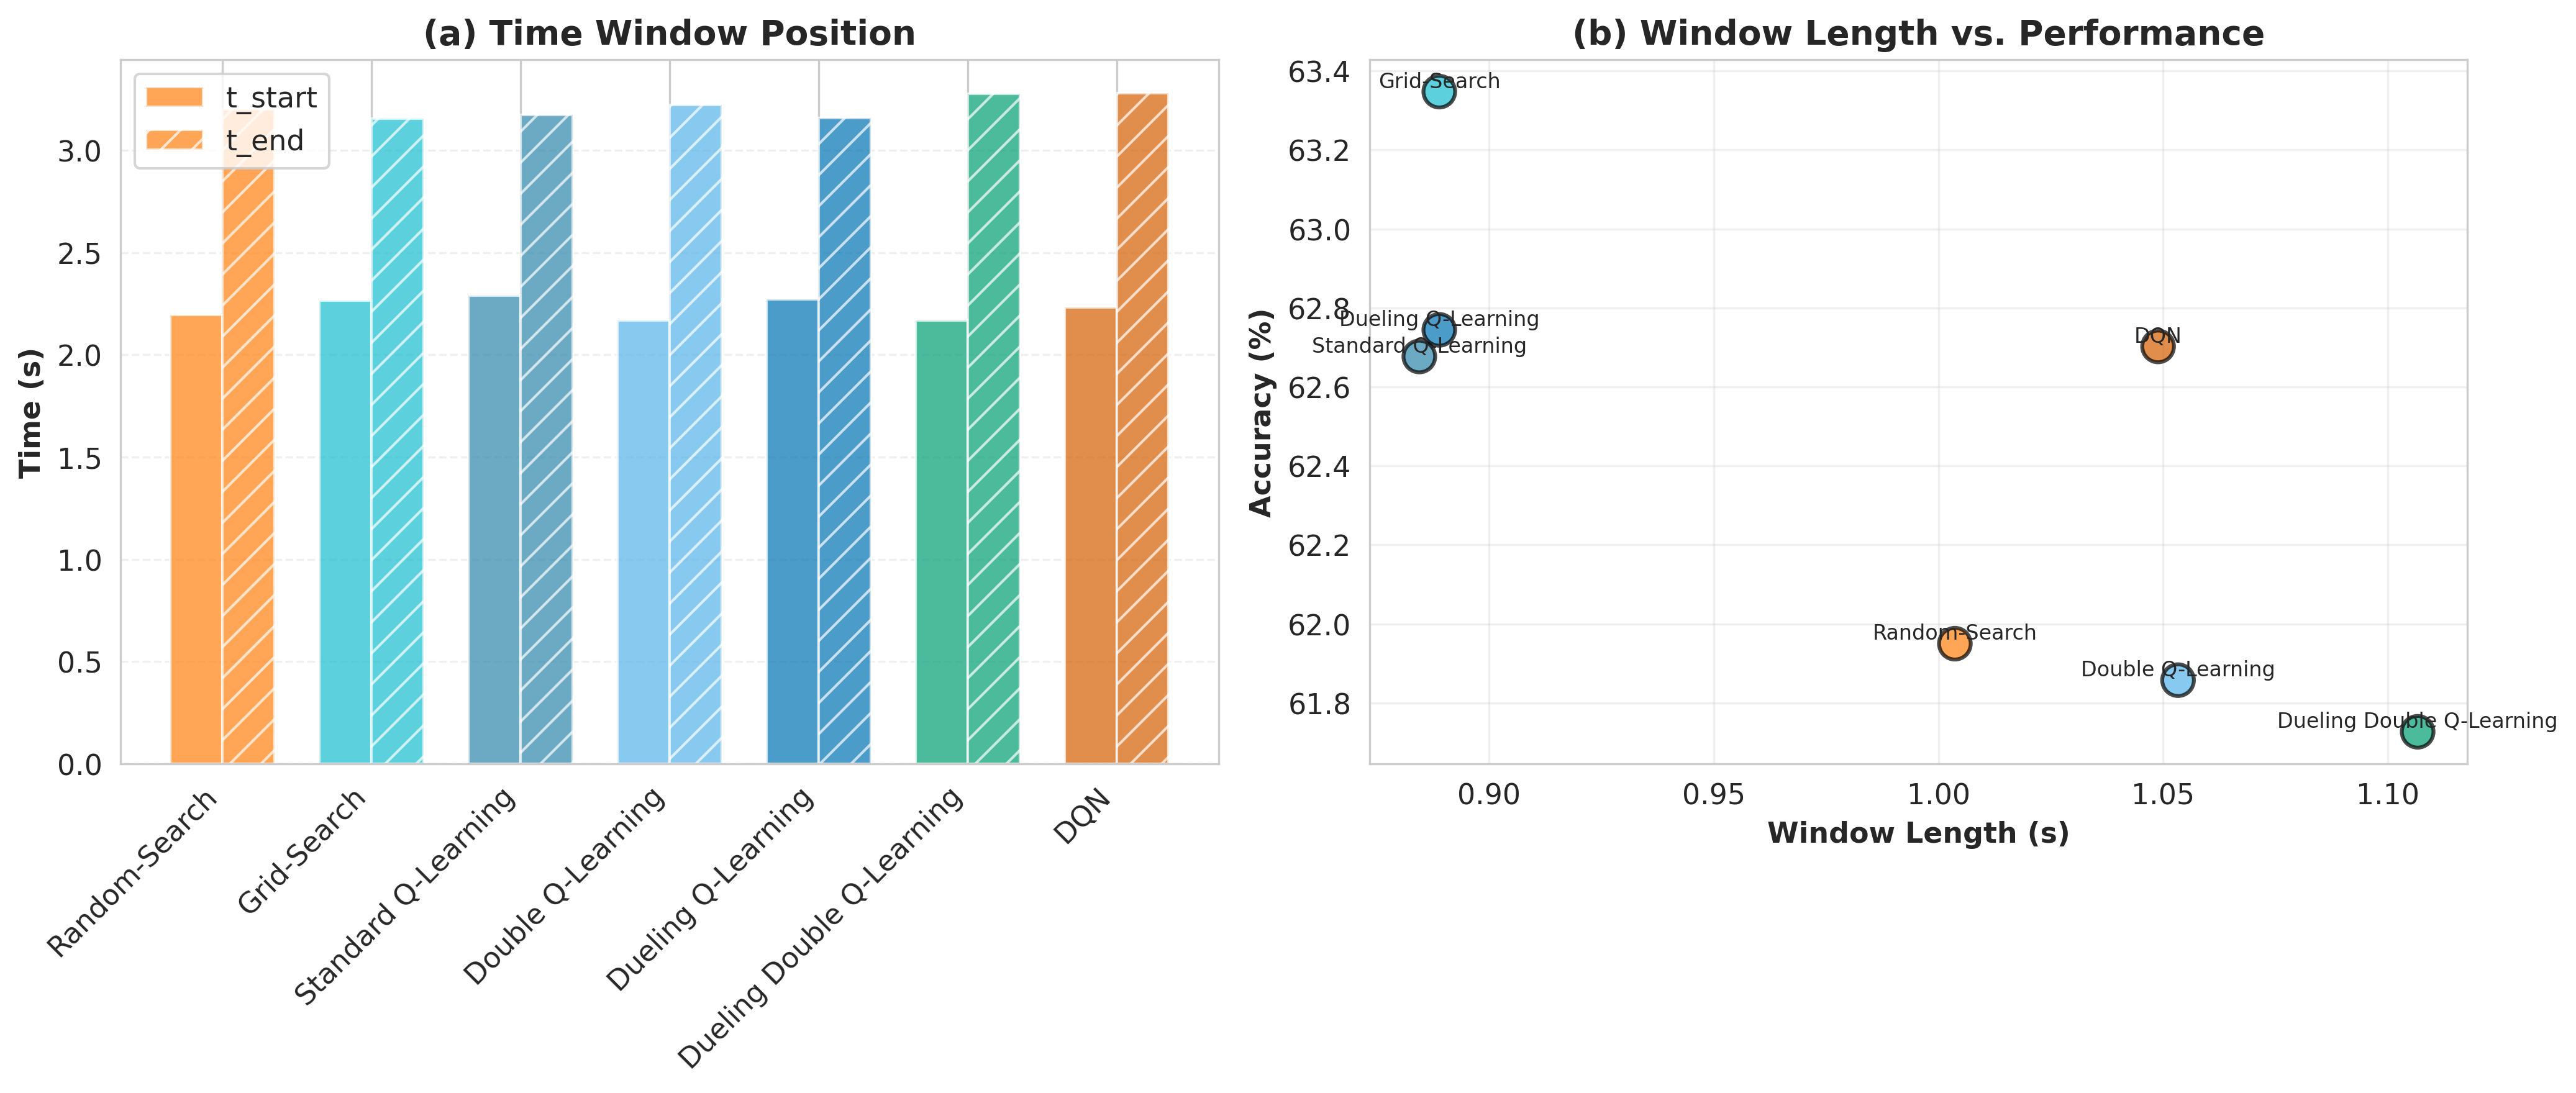
\includegraphics[height=0.7\textheight]{figures/q_vs_baseline/02_window_performance.png}
    \vspace{0.3em}
    \parbox{0.8\textwidth}{\footnotesize 图：窗口长度与性能关系散点图}
\end{frame}

% ==================== 表格型 Q-Learning 与 DQN 对比 ====================
\begin{frame}{表格型 Q-Learning vs DQN：整体性能}
    \centering
    \vspace{-0.5em}
    \begin{table}
        \centering
        \begin{tabular}{lcccccc}
            \toprule
            \textbf{Method} & \textbf{Acc (\%)} & \textbf{Kappa} & \textbf{F1} & \textbf{Std (\%)} & \textbf{$t_{start}$} & \textbf{$t_{end}$} \\
            \midrule
            \rowcolor{lightblue}
            \textbf{\color{primaryblue}Standard Q-Learning} & \textbf{62.68} & 0.5019 & 0.6201 & \textbf{8.20} & 2.29 & 3.17 \\
            DQN & \textbf{62.70} & 0.5022 & 0.6200 & 9.21 & 2.23 & 3.28 \\
            \textbf{Δ (Q - DQN)} & \textbf{-0.02} & -0.0003 & +0.0001 & \textbf{-1.01} & +0.06 & -0.11 \\
            \bottomrule
        \end{tabular}
    \end{table}

    \vspace{0.5em}

    \begin{alertblock}{\normalsize 核心发现}
        \begin{itemize}
            \item \textbf{\color{accentgreen}准确率差异极小}：仅 -0.02\%，统计学上可忽略
            \item \textbf{\color{accentgreen}稳定性优势}：标准差相对降低 10.97\%
            \item \textbf{时间窗选择}：Table Q 选择更短但信息密度更高的窗口 (0.88s vs 1.05s)
        \end{itemize}
    \end{alertblock}
\end{frame}

\begin{frame}{Table Q vs DQN 性能对比（可视化）}
    \centering
    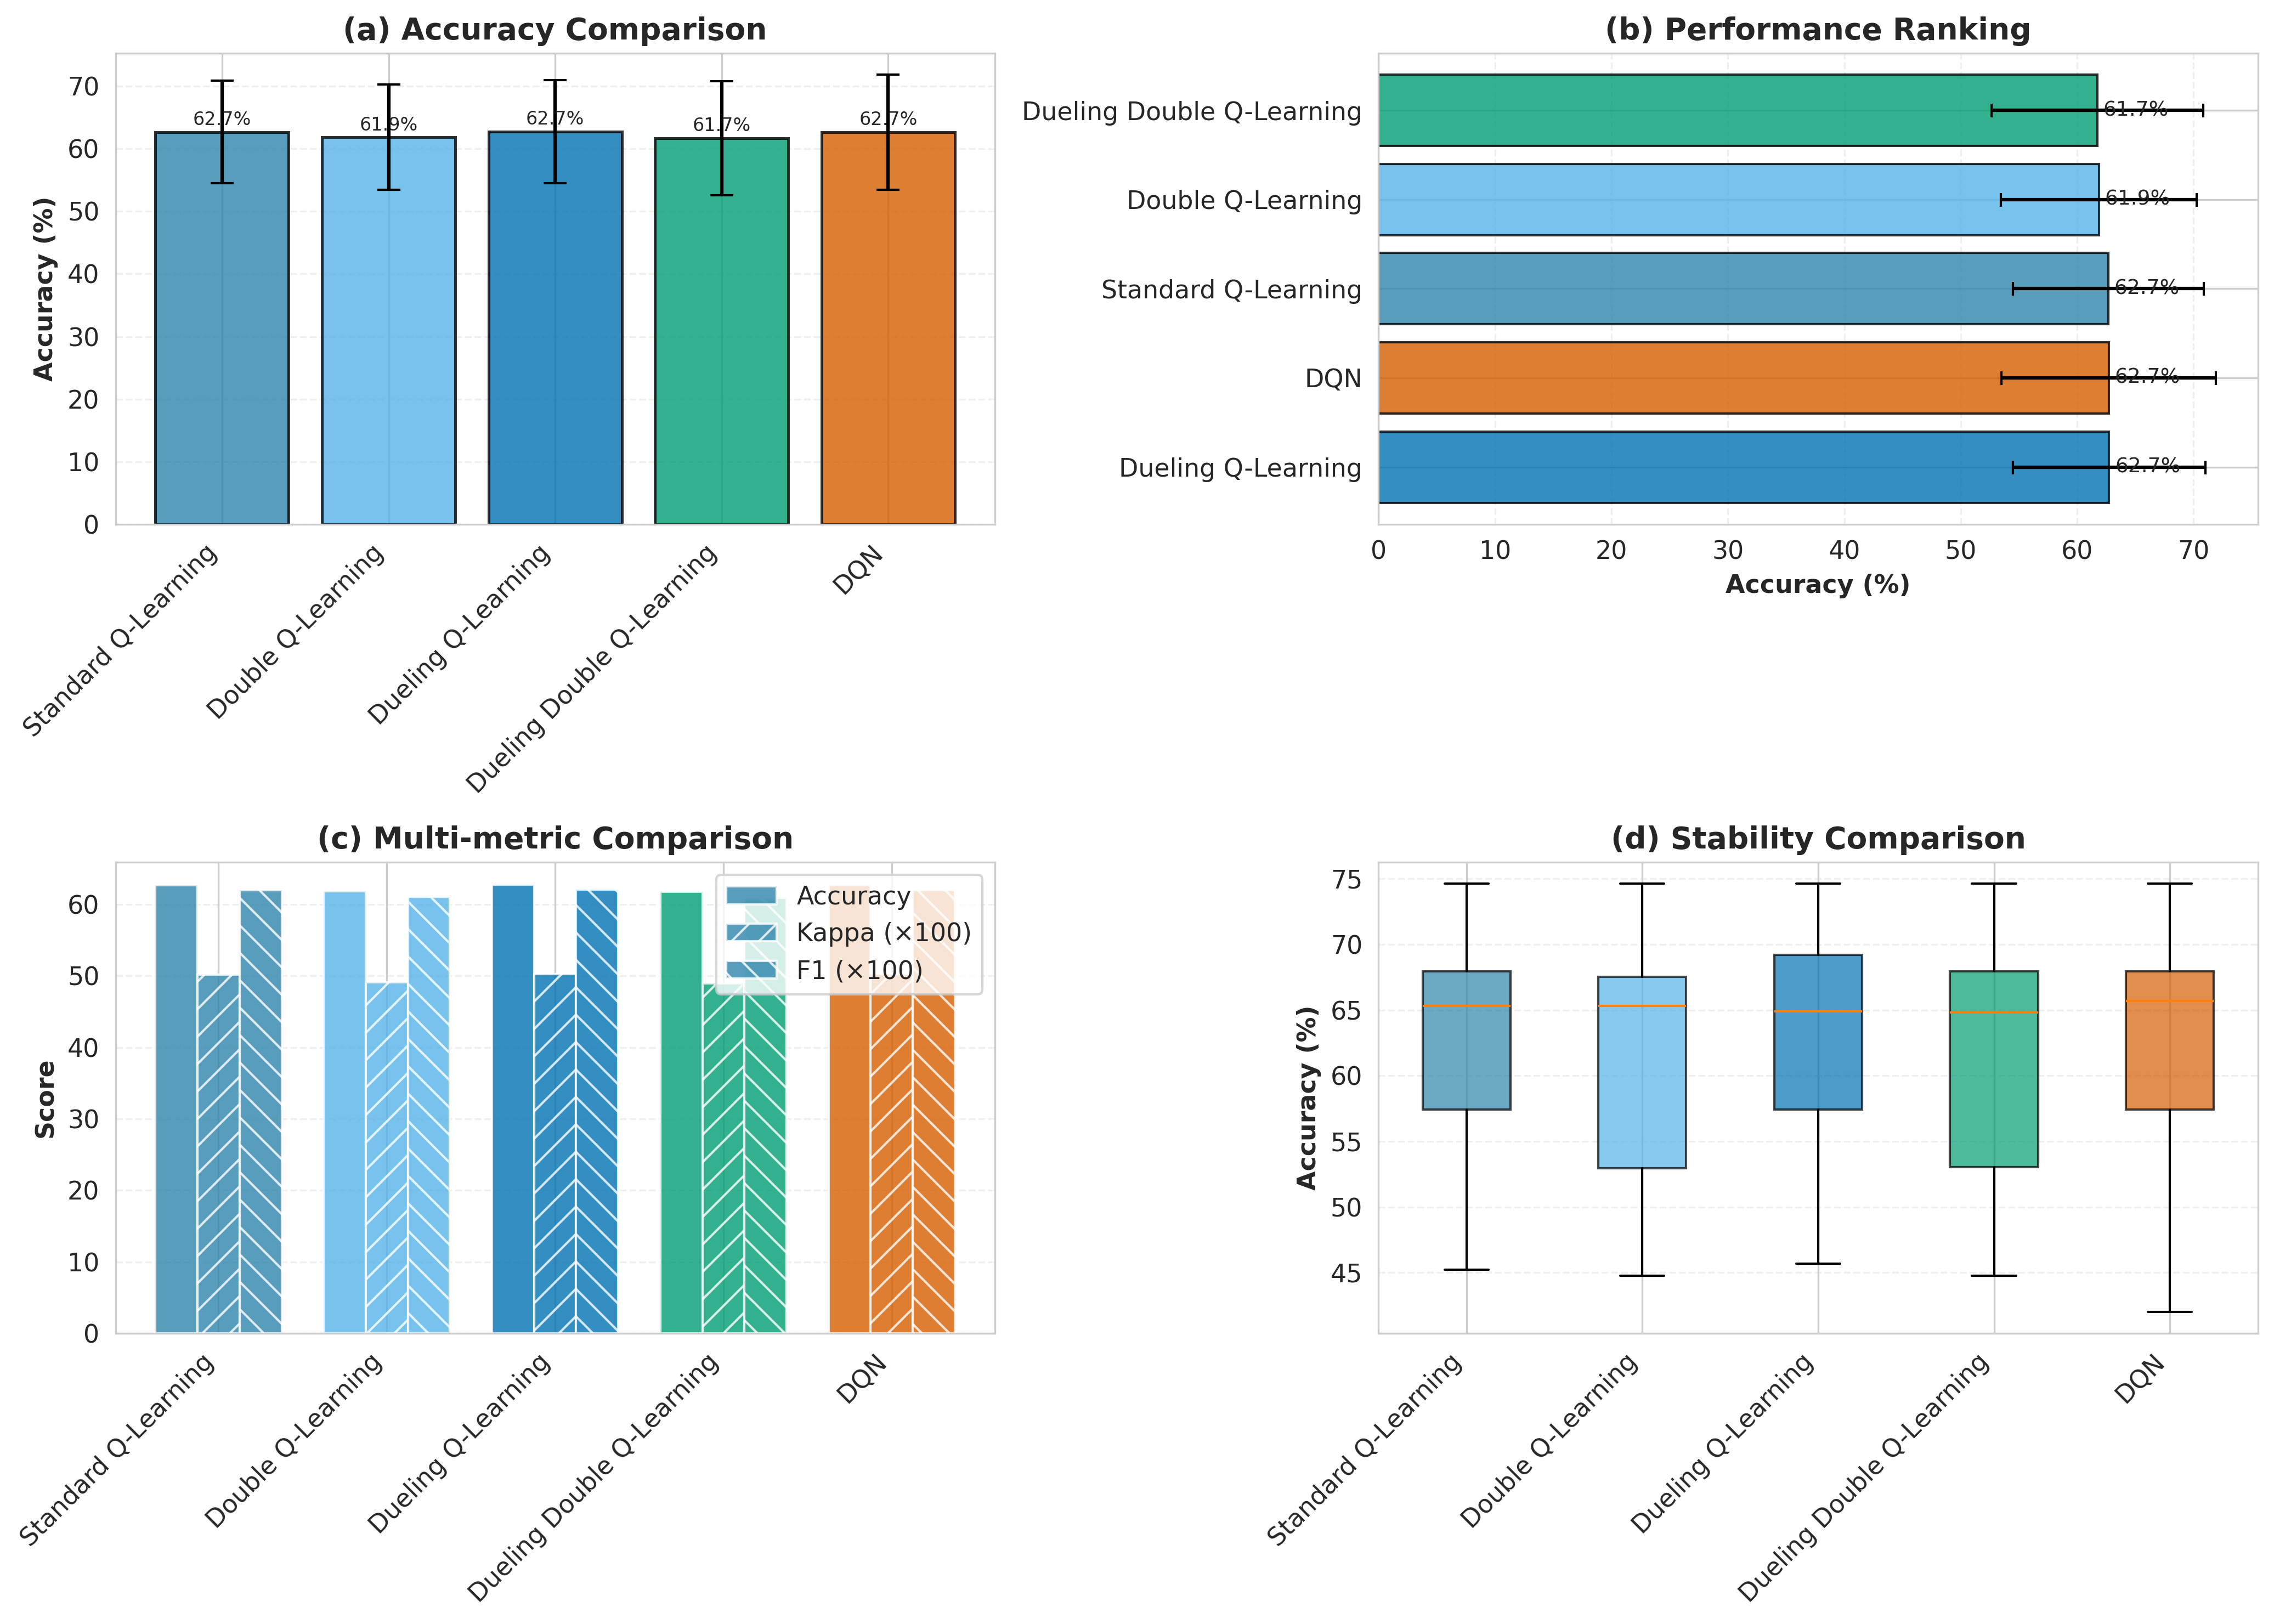
\includegraphics[height=0.7\textheight]{figures/q_internal/03_performance_comparison.png}
    \vspace{0.3em}
    \parbox{0.8\textwidth}{\footnotesize 图：Table Q vs DQN 性能对比}
\end{frame}

\begin{frame}{被试级别性能对比}
    \centering
    \vspace{-0.5em}
    \begin{table}
        \centering
        \footnotesize
        \begin{tabular}{lcccccc}
            \toprule
            \textbf{Sub} & \textbf{Table Q} & \textbf{DQN} & \textbf{Δ} & \textbf{Table Q $\kappa$} & \textbf{DQN $\kappa$} & \textbf{Δ$\kappa$} \\
            \midrule
            S01 & 64.47 & 65.71 & -1.24 & 0.5260 & 0.5435 & -0.018 \\
            \rowcolor{lightblue}
            S02 & 58.37 & 56.74 & +1.63 & 0.4780 & 0.4233 & +0.055 \\
            S03 & 68.89 & 71.70 & -2.81 & 0.5849 & 0.6226 & -0.038 \\
            \rowcolor{lightblue}
            S04 & 51.91 & 51.15 & +0.76 & 0.3590 & 0.3469 & +0.012 \\
            S05 & 65.42 & 65.27 & +0.15 & 0.5389 & 0.5368 & +0.002 \\
            \rowcolor{lightblue}
            S06 & 47.03 & 45.21 & +1.82 & 0.2952 & 0.2625 & +0.033 \\
            S07 & 65.46 & 65.61 & -0.15 & 0.5395 & 0.5416 & -0.002 \\
            \rowcolor{lightblue}
            S08 & 73.56 & 74.62 & -1.06 & 0.6470 & 0.6611 & -0.014 \\
            S09 & 68.69 & 68.27 & +0.42 & 0.5824 & 0.5769 & +0.006 \\
            \bottomrule
        \end{tabular}
    \end{table}

    \vspace{0.3em}

    \begin{exampleblock}{\normalsize 发现}
        \begin{itemize}
            \item \textbf{优劣分布均衡}：Table Q 在 5 名被试上优于或持平 DQN
            \item \textbf{低表现被试优势}：S06 上 Table Q 优于 DQN (+1.82\%)
            \item \textbf{高表现被试差距小}：S03、S08 差距 < 3\%
        \end{itemize}
    \end{exampleblock}
\end{frame}

\begin{frame}{被试级别性能对比（可视化）}
    \centering
    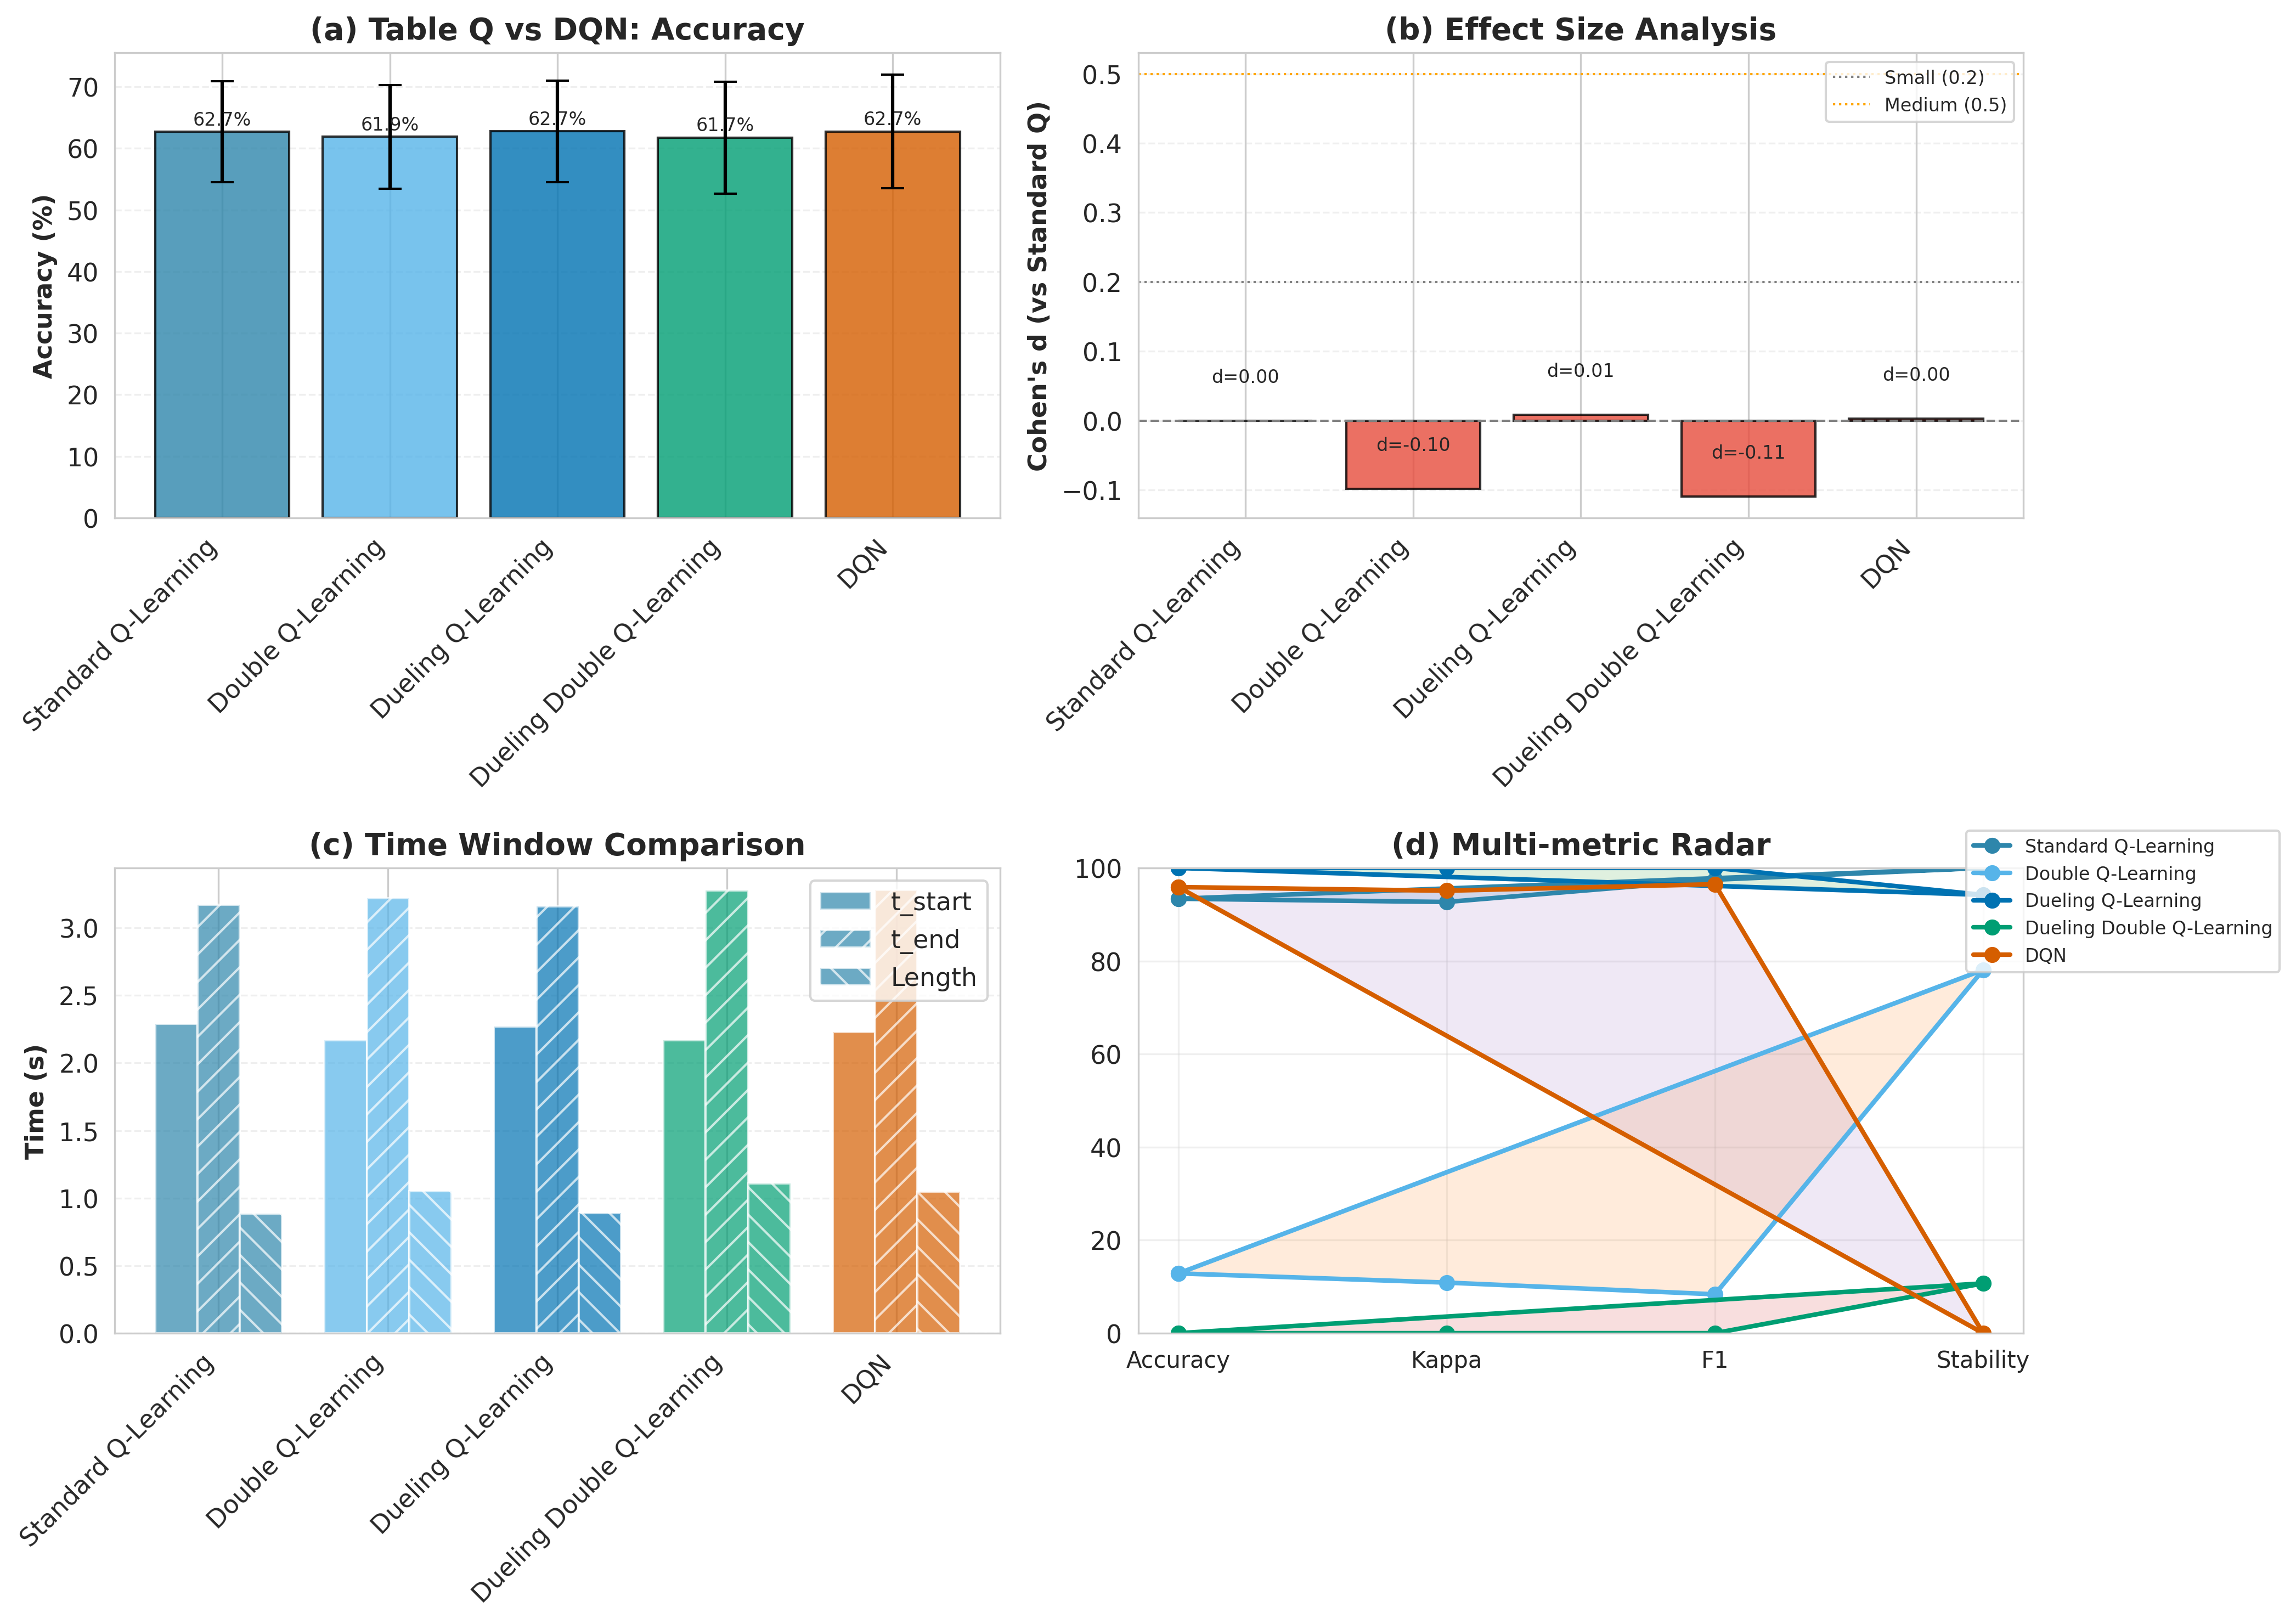
\includegraphics[height=0.7\textheight]{figures/q_internal/03_table_q_vs_dqn.png}
    \vspace{0.3em}
    \parbox{0.8\textwidth}{\footnotesize 图：被试级别性能对比}
\end{frame}

\begin{frame}{统计显著性检验}
    \begin{columns}[T]
        \begin{column}{0.48\textwidth}
            \begin{alertblock}{\normalsize 配对样本 t 检验}
                \begin{itemize}
                    \item \textbf{零假设} $H_0$：$\mu_d = 0$（无显著差异）
                    \item \textbf{备择假设} $H_1$：$\mu_d \neq 0$
                \end{itemize}

                \vspace{0.5em}

                \textbf{检验结果}：
                \begin{itemize}
                    \item $t$ 统计量：$t(8) = \textbf{-0.024}$
                    \item $p$ 值：\textbf{\color{accentgreen}$p = 0.981$}
                    \item 95\% CI：$[-2.01\%, 1.97\%]$
                    \item Cohen's $d = \textbf{-0.003}$
                \end{itemize}
            \end{alertblock}
        \end{column}

        \begin{column}{0.48\textwidth}
            \begin{exampleblock}{\normalsize 结果解读}
                \begin{itemize}
                    \item $p = 0.981 > 0.05$，\textbf{\color{accentgreen}不能拒绝零假设}
                    \item 效应量 $d = -0.003$ 远小于 0.2
                    \item \textbf{结论}：两种方法性能差异在统计学上不显著
                \end{itemize}
            \end{exampleblock}
        \end{column}
    \end{columns}
\end{frame}

\begin{frame}{模型训练性能可视化}
    \centering
    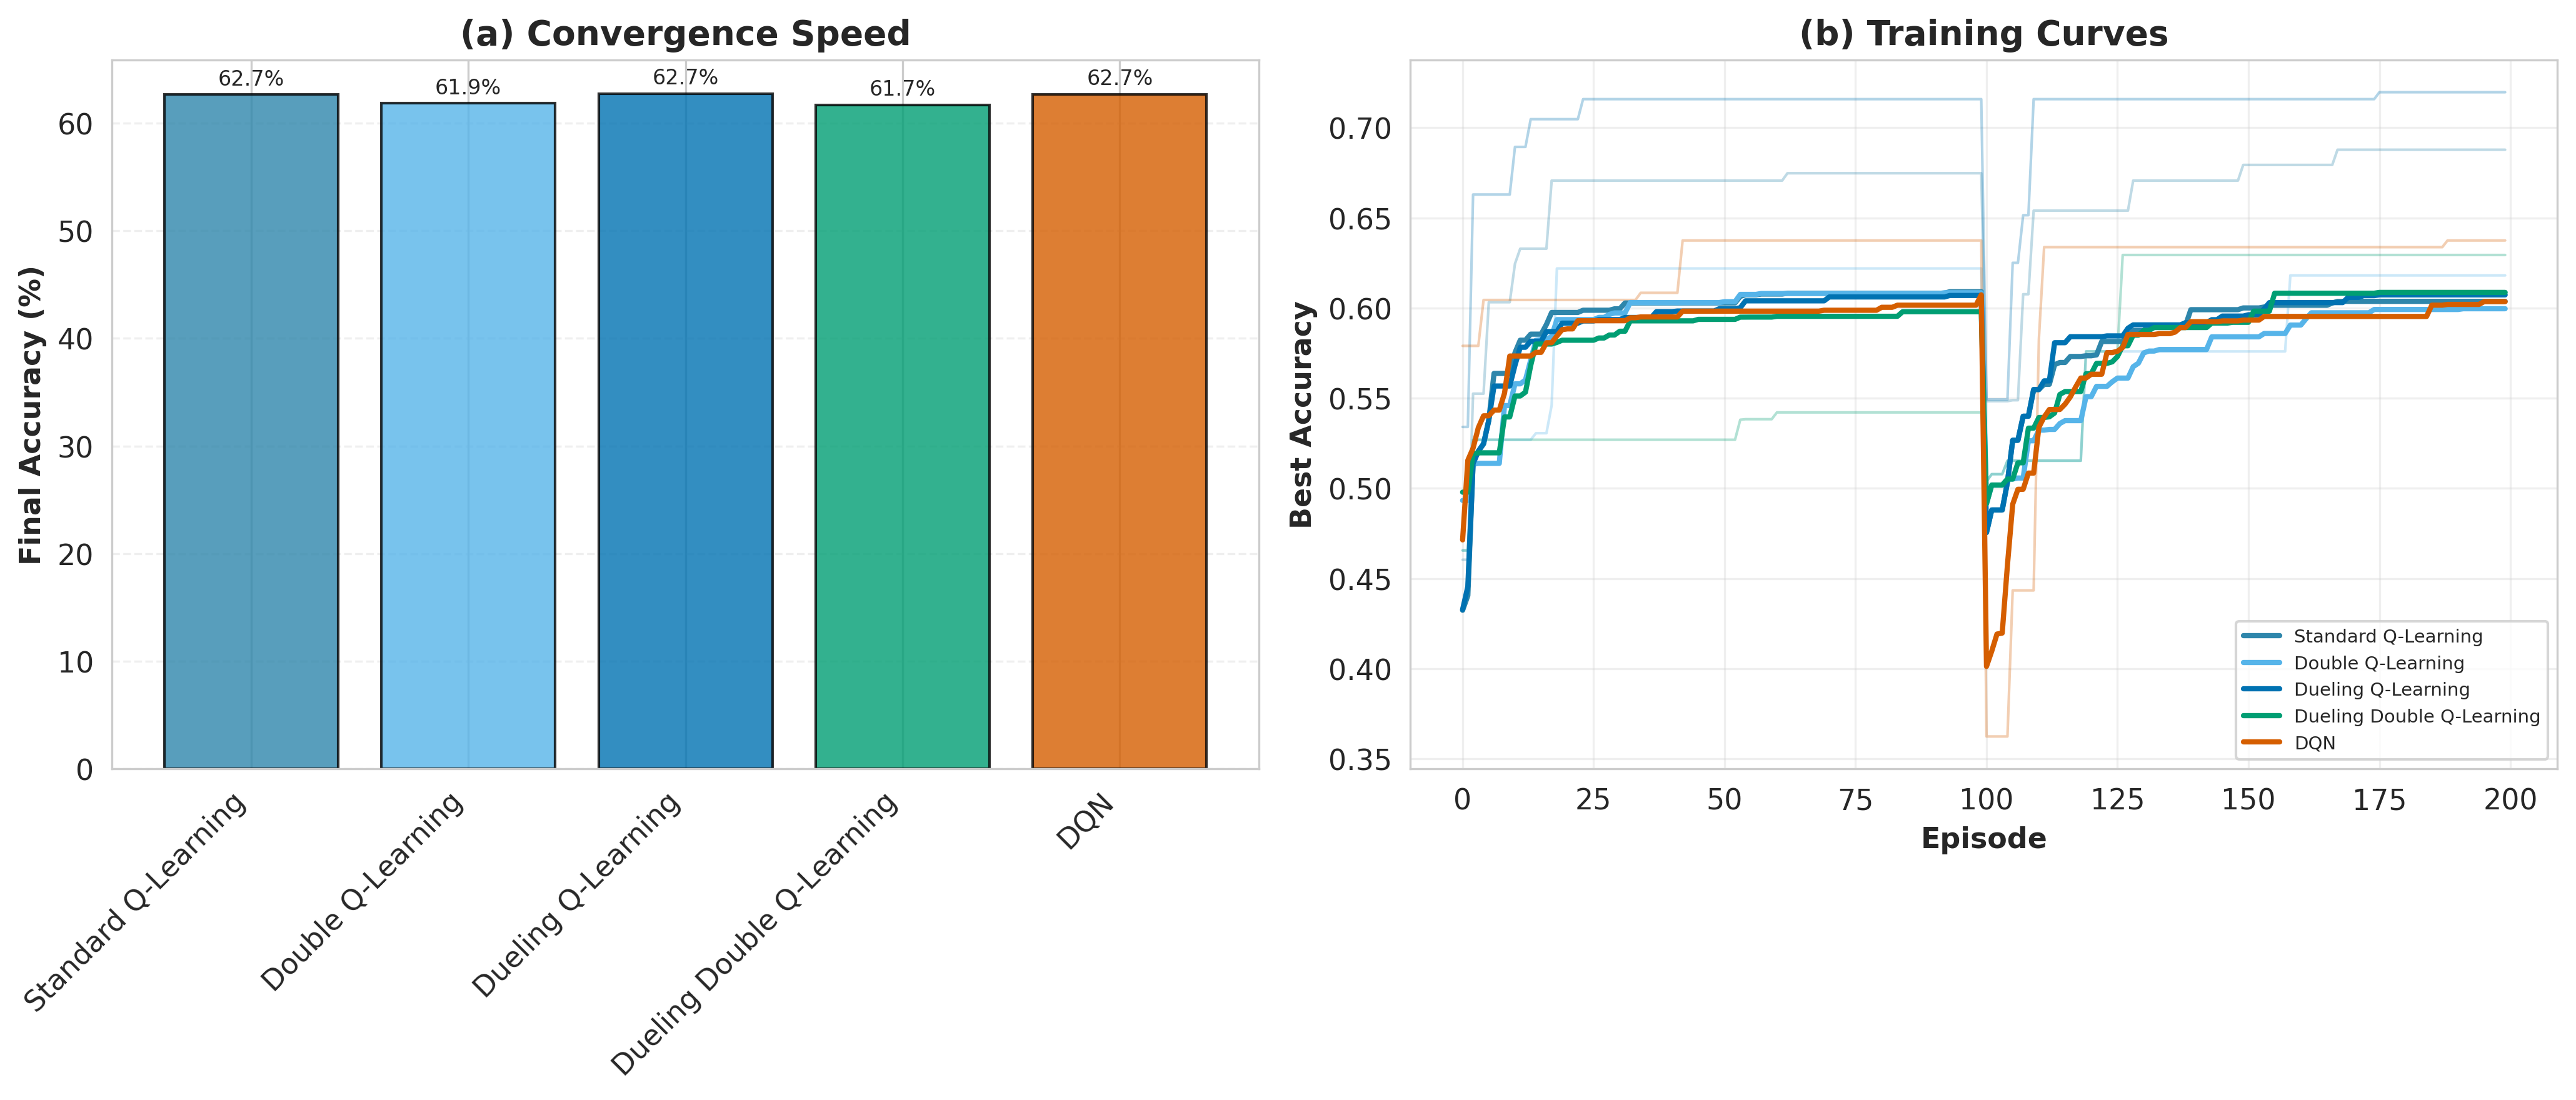
\includegraphics[height=0.7\textheight]{figures/q_internal/03_training_performance.png}
    \vspace{0.3em}
    \parbox{0.8\textwidth}{\footnotesize 图：训练性能对比}
\end{frame}

% ==================== 消融实验 ====================
\begin{frame}{Q-Learning 变体消融实验}
    \centering
    \vspace{-0.5em}
    \begin{table}
        \centering
        \begin{tabular}{lcccc}
            \toprule
            \textbf{Method} & \textbf{Acc (\%)} & \textbf{Δ Acc} & \textbf{Effect Size} & \textbf{Std (\%)} \\
            \midrule
            \rowcolor{lightblue}
            \textbf{\color{primaryblue}Standard Q-Learning} & \textbf{62.68} & \textbf{+0.00} & \textbf{0.00} & \textbf{8.20} \\
            Double Q-Learning & 61.86 & -1.31 & -0.10 & 8.42 \\
            \rowcolor{lightblue}
            Dueling Q-Learning & 62.74 & +0.11 & +0.01 & 8.26 \\
            Dueling Double Q & 61.73 & -1.52 & -0.11 & 9.11 \\
            \rowcolor{lightblue}
            DQN & 62.70 & +0.02 & +0.01 & 9.21 \\
            \bottomrule
        \end{tabular}
    \end{table}


    \begin{alertblock}{\normalsize 消融实验结论}
        \begin{itemize}
            \item \textbf{\color{accentgreen}Standard Q-Learning 最优}：准确率 62.68\%，稳定性最佳
            \item \textbf{Double Q-Learning 未带来收益}：准确率下降 1.31\%
            \item \textbf{Dueling 架构效果有限}：准确率微幅提升 0.11\%
            \item \textbf{组合效果不佳}：Dueling Double Q 下降 1.52\%
        \end{itemize}
    \end{alertblock}
\end{frame}

\begin{frame}{消融实验：性能演化}
    \centering
    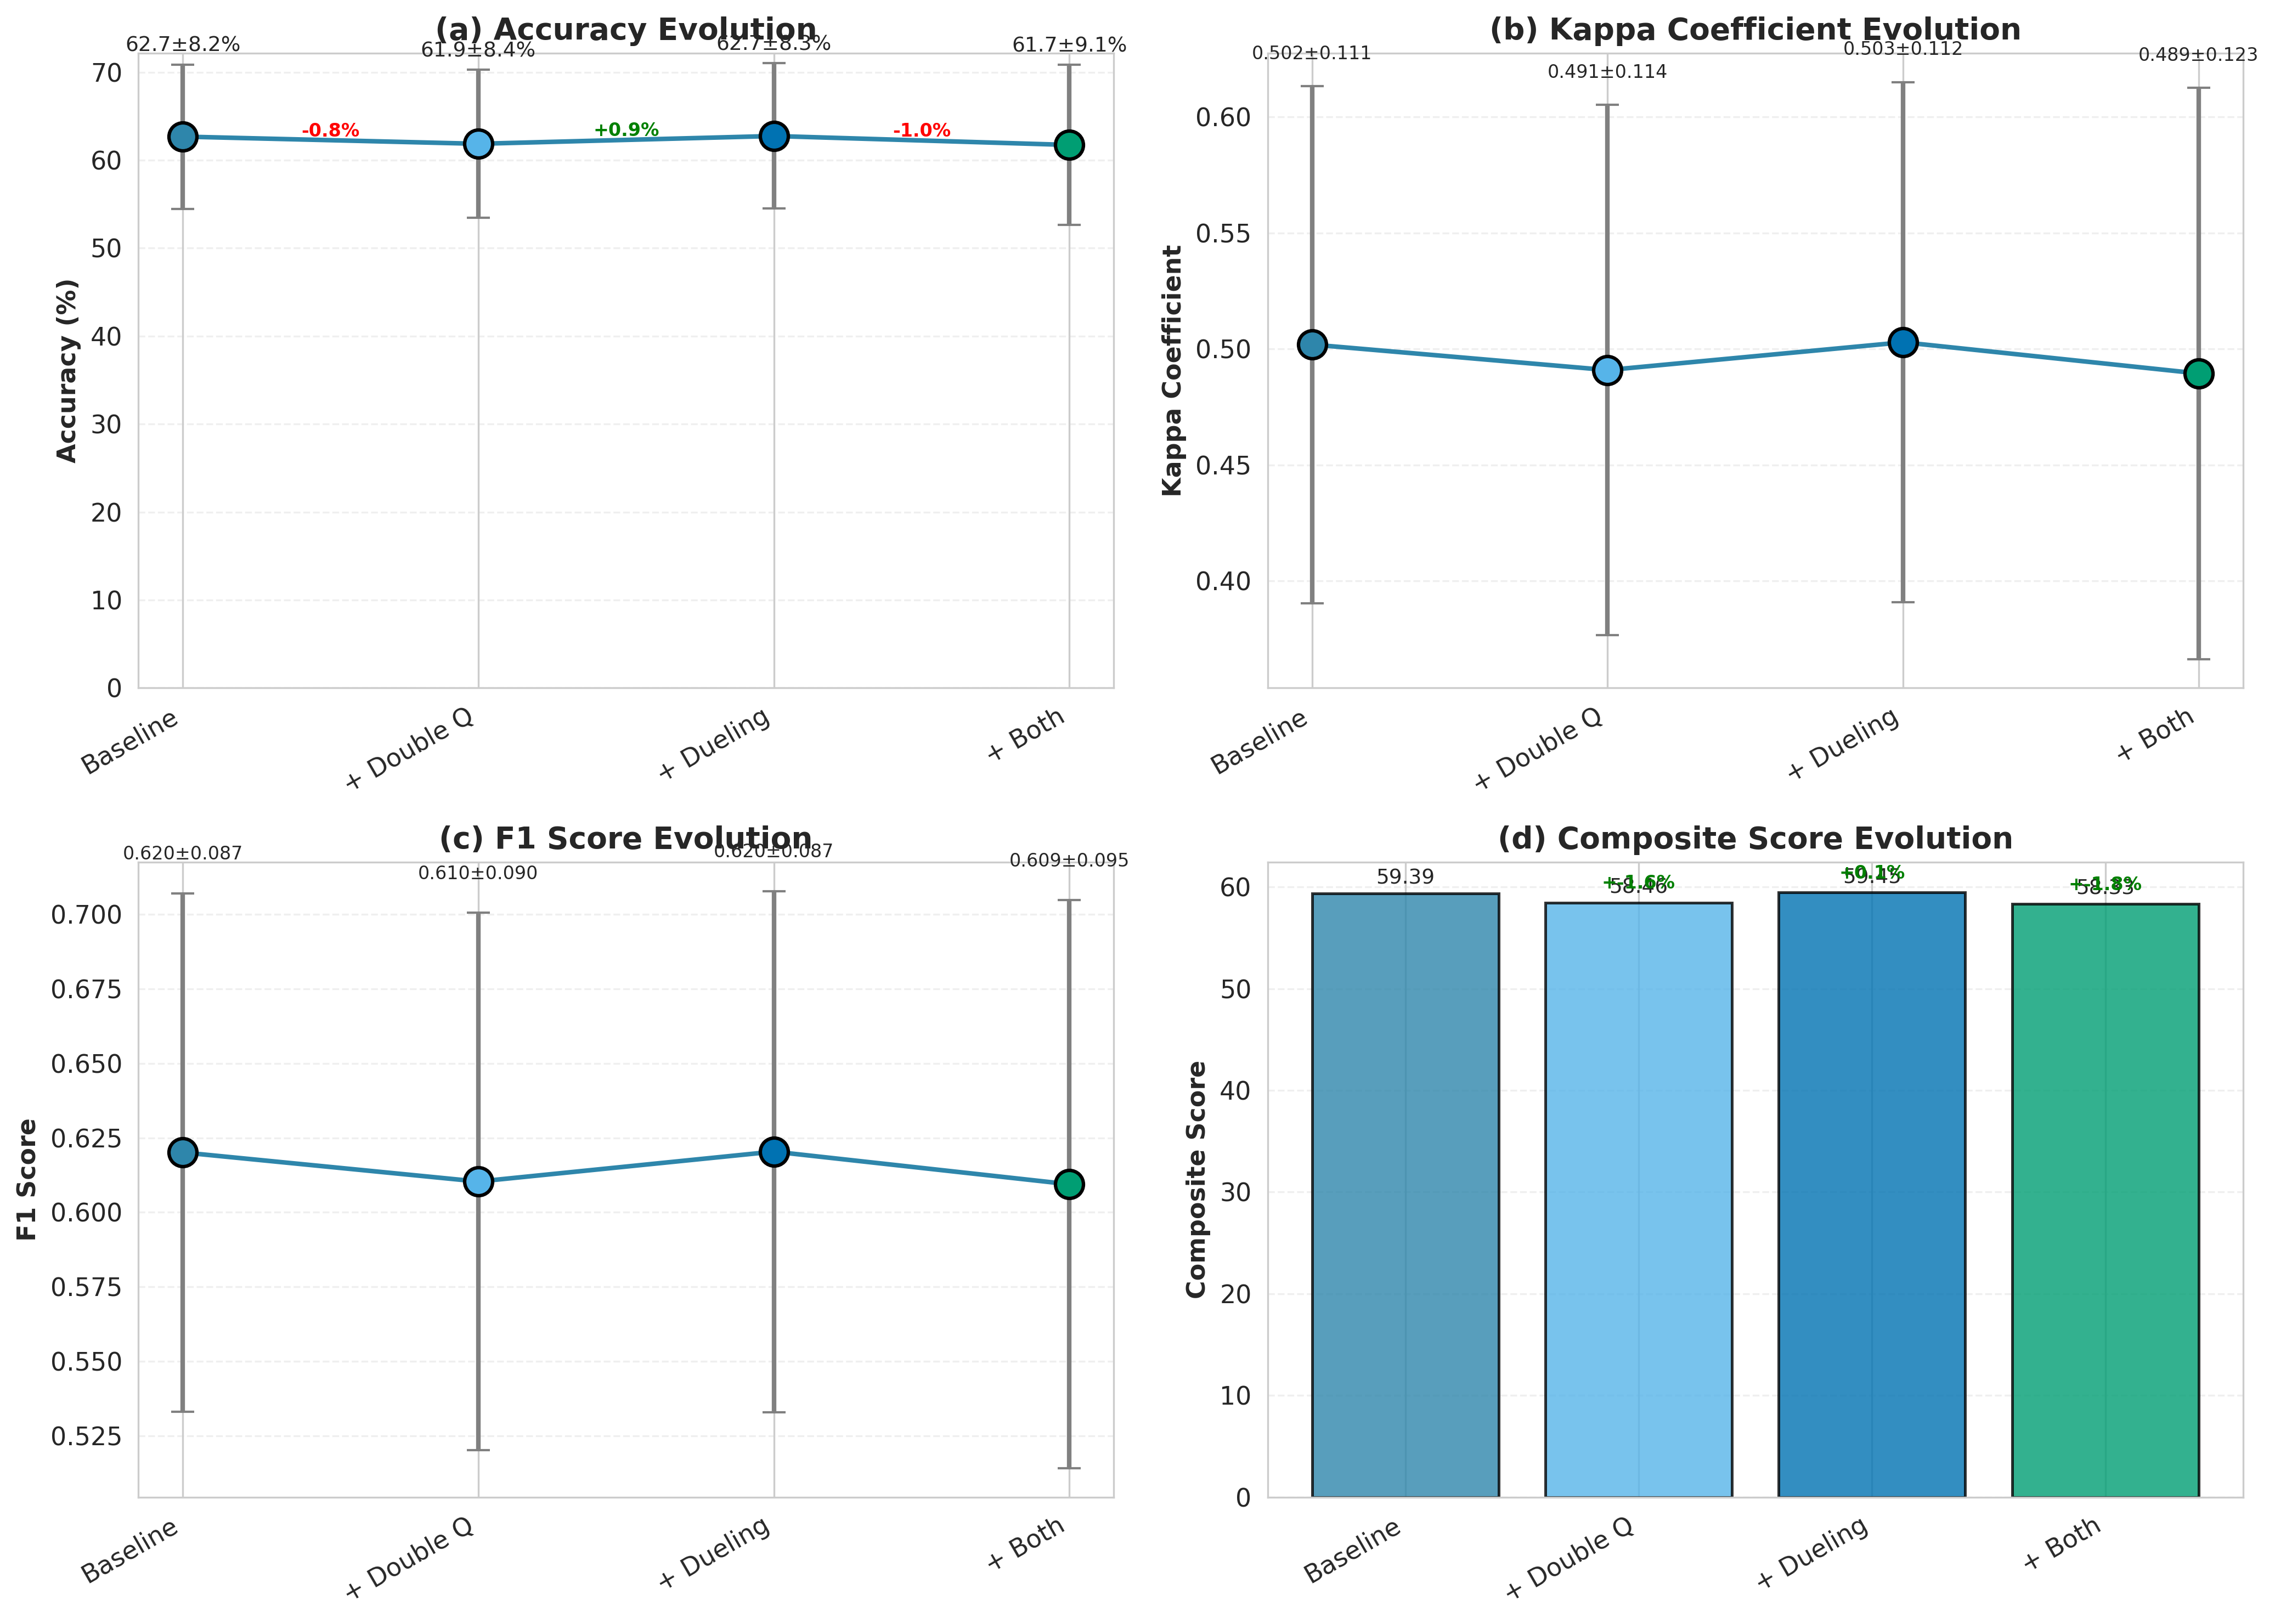
\includegraphics[height=0.7\textheight]{figures/ablation/04_performance_evolution.png}
    \vspace{0.3em}
    \parbox{0.8\textwidth}{\footnotesize 图：各变体性能演化对比}
\end{frame}

\begin{frame}{消融实验：时间窗演化}
    \centering
    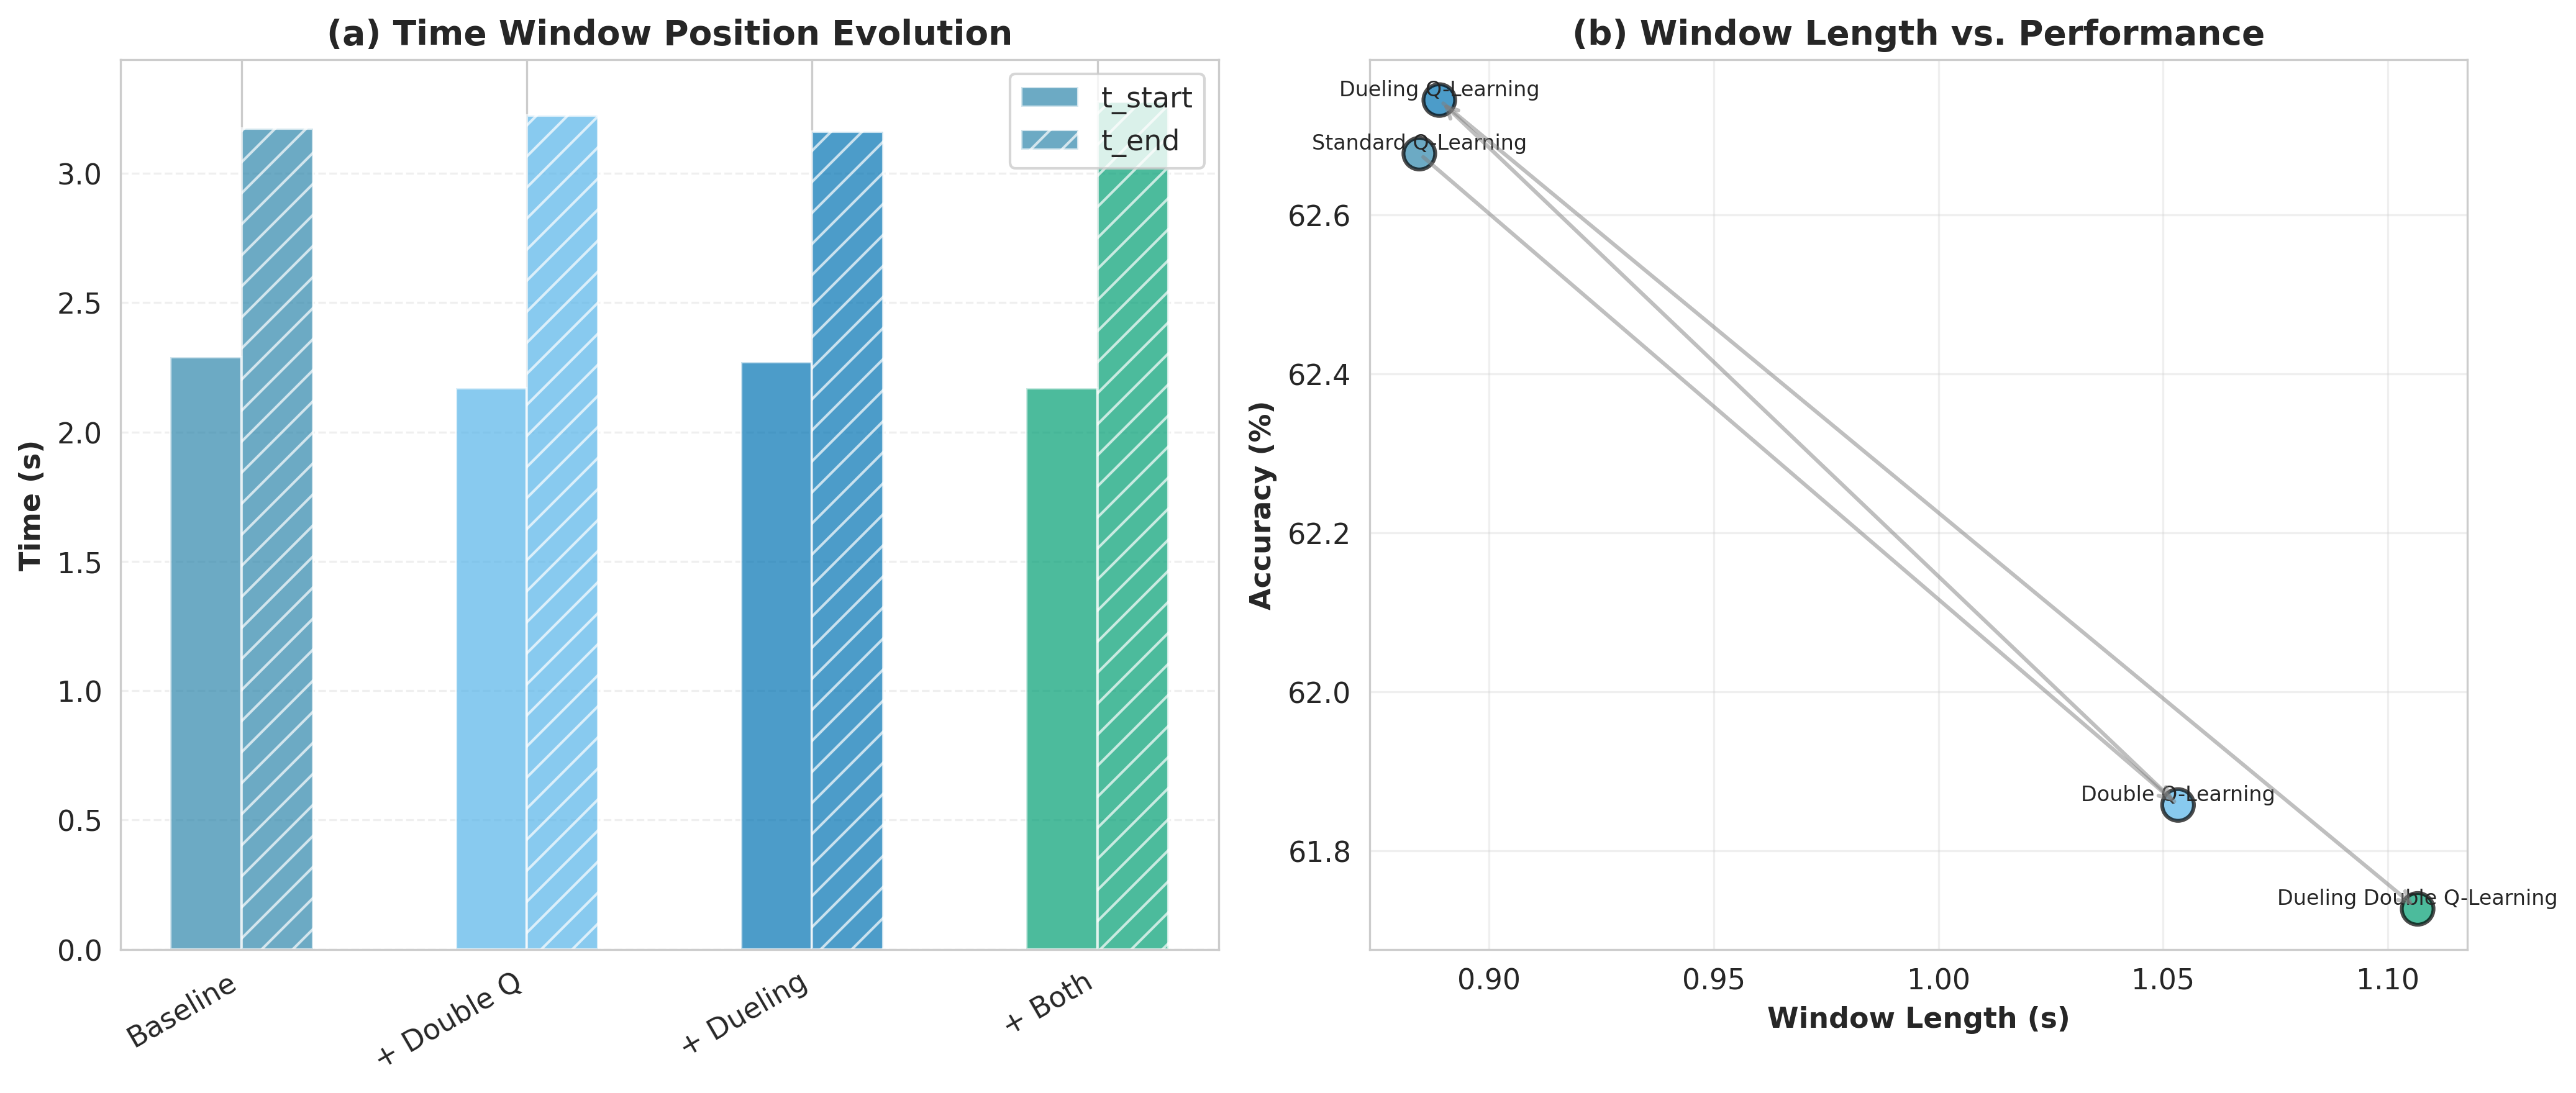
\includegraphics[height=0.7\textheight]{figures/ablation/04_window_evolution.png}
    \vspace{0.3em}
    \parbox{0.8\textwidth}{\footnotesize 图：各变体时间窗选择演化}
\end{frame}

\begin{frame}{消融实验：性能提升分析}
    \centering
    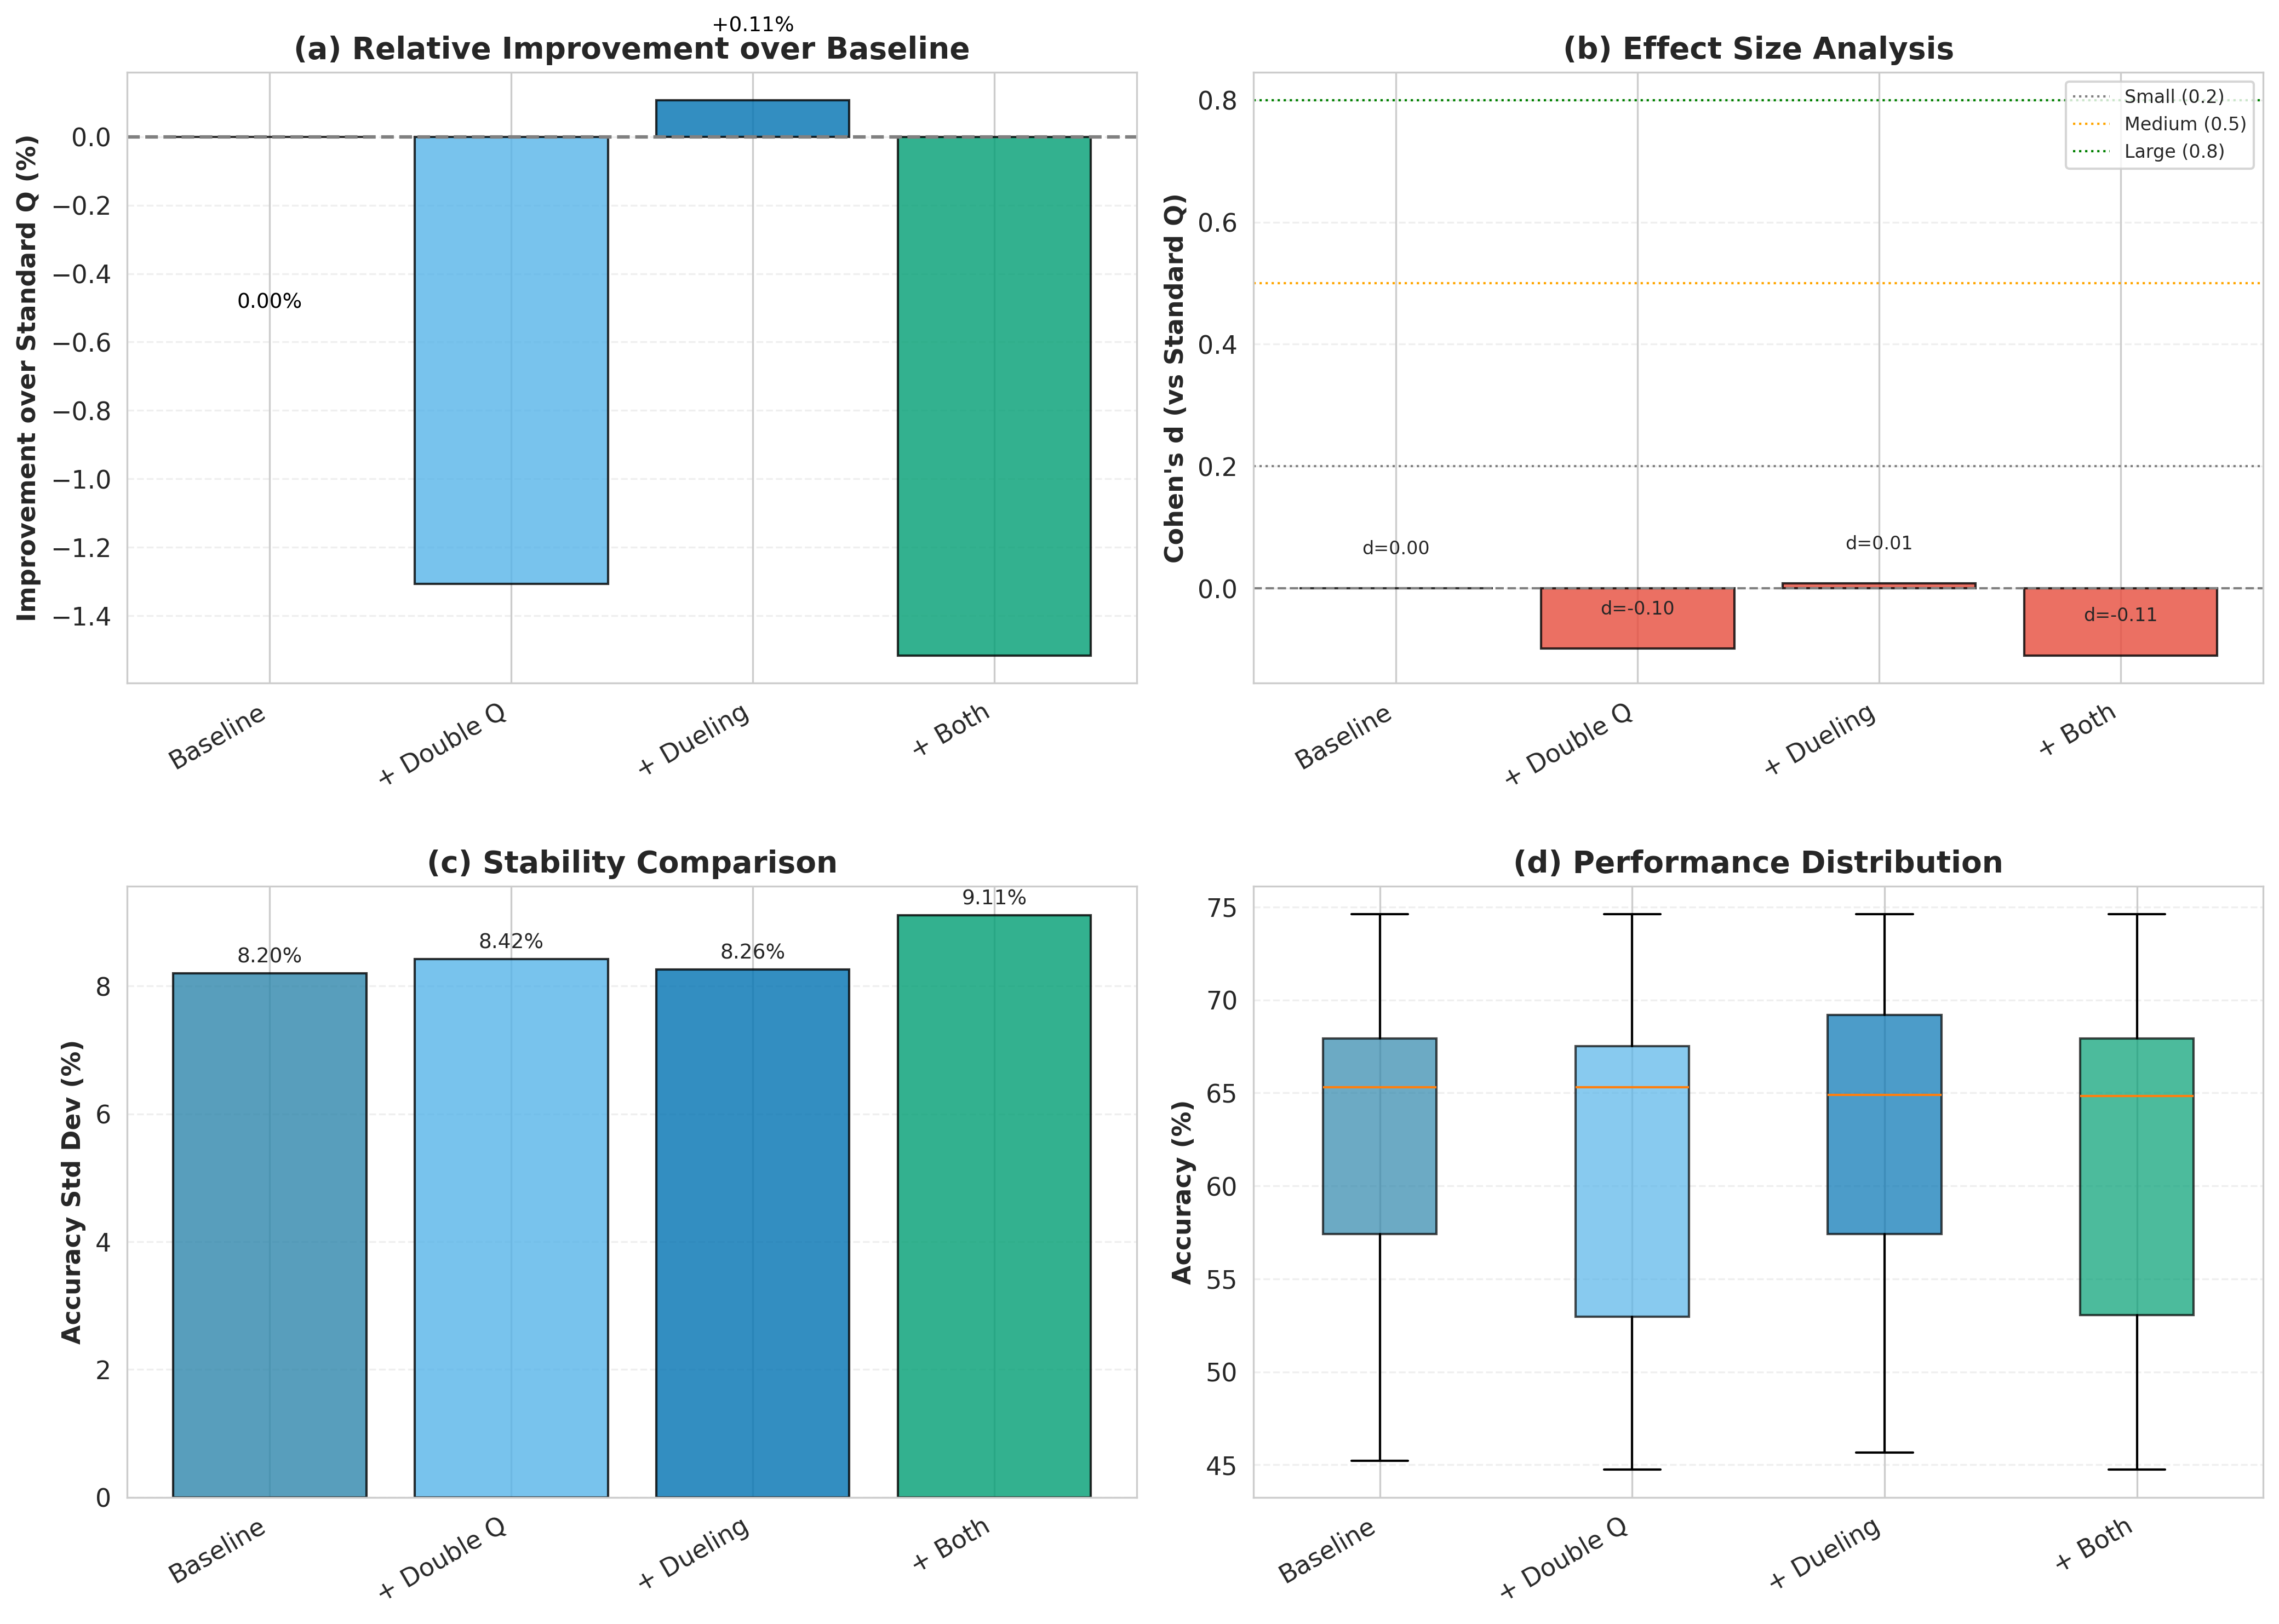
\includegraphics[height=0.8\textheight]{figures/ablation/04_improvement_analysis.png}
    \vspace{0.3em}
    \parbox{0.8\textwidth}{\footnotesize 图：性能提升分析}


\end{frame}

% ==================== 自适应 vs 固定时间窗 ====================
\begin{frame}{自适应时间窗 vs 固定时间窗 (S01 被试)}
    \centering
    \vspace{-0.5em}
    \begin{table}
        \centering
        \begin{tabular}{lccccc}
            \toprule
            \textbf{Method} & \textbf{Type} & \textbf{$t_{start}$} & \textbf{$t_{end}$} & \textbf{Length} & \textbf{Acc (\%)} \\
            \midrule
            FL-1s & Fixed & 2.5 & 3.5 & 1.0 & 61.54 \\
            \rowcolor{lightblue}
            FL-1.5s & Fixed & 2.5 & 4.0 & 1.5 & 59.34 \\
            FL-2s & Fixed & 2.0 & 4.0 & 2.0 & 57.88 \\
            \rowcolor{lightblue}
            \textbf{\color{primaryblue}Standard Q-Learning} & \textbf{Adaptive} & \textbf{2.80} & \textbf{3.60} & \textbf{0.80} & \textbf{65.93} \\
            \bottomrule
        \end{tabular}
    \end{table}

    \vspace{0.5em}

    \begin{alertblock}{\normalsize 关键发现}
        \begin{itemize}
            \item \textbf{自适应优于固定}：65.93\% > 61.54\%（最佳固定窗口）
            \item \textbf{个体化选择}：为 S01 选择最优 [2.80s, 3.60s]
            \item \textbf{连续空间搜索}：不局限于预定义离散候选
        \end{itemize}
    \end{alertblock}
\end{frame}

% ==================== 被试间差异分析 ====================
\begin{frame}{被试间差异分析}
    \centering
    \vspace{-0.5em}
    \begin{table}
        \centering
        \footnotesize
        \begin{tabular}{lcccccc}
            \toprule
            \textbf{Sub} & \textbf{Acc (\%)} & \textbf{Kappa} & \textbf{F1} & \textbf{$t_{start}$} & \textbf{$t_{end}$} & \textbf{Length} \\
            \midrule
            S01 & 64.47 & 0.5260 & 0.6446 & 2.68 & 3.56 & 0.88 \\
            \rowcolor{lightblue}
            S02 & 58.37 & 0.4780 & 0.5919 & 2.16 & 2.96 & 0.80 \\
            S03 & 68.89 & 0.5849 & 0.6889 & 2.36 & 3.72 & 1.36 \\
            \rowcolor{lightblue}
            S04 & 51.91 & 0.3590 & 0.5209 & 2.04 & 2.64 & 0.60 \\
            S05 & 65.42 & 0.5389 & 0.6484 & 2.00 & 2.68 & 0.68 \\
            \rowcolor{lightblue}
            S06 & 47.03 & 0.2952 & 0.4415 & 2.00 & 2.88 & 0.88 \\
            S07 & 65.46 & 0.5395 & 0.6528 & 2.04 & 2.92 & 0.88 \\
            \rowcolor{lightblue}
            S08 & 73.56 & 0.6470 & 0.7293 & 2.44 & 3.92 & 1.48 \\
            S09 & 68.69 & 0.5824 & 0.6784 & 2.68 & 3.36 & 0.68 \\
            \midrule
            \textbf{Mean} & \textbf{62.68} & \textbf{0.5019} & \textbf{0.6201} & \textbf{2.29} & \textbf{3.17} & \textbf{0.88} \\
            \textbf{Std} & \textbf{8.20} & \textbf{0.1114} & \textbf{0.0869} & \textbf{0.26} & \textbf{0.46} & \textbf{0.32} \\
            \bottomrule
        \end{tabular}
    \end{table}

    \vspace{0.3em}

    \begin{columns}[T]
        \begin{column}{0.32\textwidth}
            \begin{block}{\centering \normalsize {高表现组}}
                S03, S07, S08, S09 \\
                Acc > 65\%
            \end{block}
        \end{column}
        \begin{column}{0.32\textwidth}
            \begin{alertblock}{\centering \normalsize {中表现组}}
                S01, S02, S05 \\
                Acc 58\%-65\%
            \end{alertblock}
        \end{column}
        \begin{column}{0.32\textwidth}
            \begin{exampleblock}{\centering \normalsize {低表现组}}
                S04, S06 \\
                Acc < 52\%
            \end{exampleblock}
        \end{column}
    \end{columns}
\end{frame}

